\documentclass[12pt,a4paper]{report}
%\fontencoding{T1}

\usepackage[utf8]{inputenc}
\usepackage[T1]{fontenc}
\usepackage[danish]{babel}
\usepackage[hidelinks]{hyperref}
\usepackage{lingmacros}
\usepackage{tree-dvips}
\usepackage{url}
\usepackage{array}
\usepackage{graphicx}
\usepackage{float}
\usepackage{lastpage}
\usepackage{color}
\usepackage[x11names,rgb,usenames,dvipsnames,svgnames,table]{xcolor}
\usepackage{colortbl}
\usepackage{algorithm2e}
\usepackage{geometry}
\usepackage{titlesec, blindtext, color}
\definecolor{gray75}{gray}{0.75}
\definecolor{gray90}{gray}{0.90}
\definecolor{ForestGreen}{RGB}{15,116,61}
\definecolor{gray25}{gray}{0.25}
\newcommand{\hsp}{\hspace{20pt}}

\usepackage{tikz}
\usetikzlibrary{snakes,arrows,shapes}
\usepackage{amsmath}

\usepackage{xcolor} 
\usepackage{fix-cm} 

%Titelblad fix
%\usepackage[ansinew]{inputenc}
\usepackage{a4}

\titleformat{\chapter}[hang]{\Huge\bfseries}{\thechapter\hsp\textcolor{gray75}{|}\hsp}{0pt}{\Huge\bfseries}

\begin{document}
\setcounter{page}{2}

\begin{titlepage}
\newcommand{\HRule}[1]{\hfill \rule{0.2\linewidth}{#1}} 

\definecolor{grey}{rgb}{0.9,0.9,0.9} 
\newgeometry{top=2in,bottom=1in,right=0cm,left=0cm}
\thispagestyle{empty} 

\noindent \colorbox{grey}{
	 \parbox[t]{1.0\linewidth}{
		\centering \fontsize{50pt}{80pt}\selectfont
		\vspace*{0.7cm}
		P1-Rapport \\[3pt]
        \LARGE Komprimering af korte beskeder \\ 
		\vspace*{0.7cm}
	}
}

\vfill
\flushright
\flushright \rule[10pt]{0.1pt}{160pt}  \begin{minipage}[b]{0.45\linewidth}
{
\Large
\textbf{Gruppe B228:} \\[4pt]
Bossen, Jannek Alexander Westerhof\\[.2cm]
Brämer, Kevin\\[.2cm]
Bønneland, Frederik Meyer\\[.2cm]
Joensen, Ólavur Debes\\[.2cm]
Olesen, Anders Trier\\[.2cm]
Tjell, Katrine Sofie\\[.2cm]
}
\end{minipage}

\clearpage 

%\title{P1-Rapport}
%\author{B228}
%\date{\today}
%\pagebreak
%\maketitle
%% Fjerner sidetal på forsiden
\thispagestyle{empty}
\end{titlepage}

%Hent titelblad (Som henter synopsis fra Indhold/Synopsis.tex):
\begin{titlepage}
\newgeometry{top=1in,bottom=1in,right=1in,left=1in}
\small
\begin{nopagebreak}
{\samepage 
\begin{tabular}{r}
\parbox{\textwidth}{  \raisebox{11mm}{
\includegraphics[height=1.2cm]{Billeder/aau-logo.pdf}}
\hfill \begin{tabular}{l}
{\sf\small \textbf{Det Teknisk-Naturvidenskabelige Basis{\aa}r }}\\
{\sf\small  \textbf{Datalogi og Software}} \\
{\sf\small Strandvejen 12-14} \\
{\sf\small Telefon 96 35 97 31} \\
{\sf\small Fax 98 13 63 93} \\
{\sf\small http://tnb.aau.dk}
\end{tabular}}
\\
\end{tabular}

\begin{tabular}{cc}
\parbox{7cm}{
\begin{description}

\item {\bf Titel:} 

Komprimering af kort tekstbesked
  
\item {\bf Tema:} 

Fra eksisterende software til modeller

\end{description}

\parbox{8cm}{

\begin{description}
\item {\bf Projektperiode:}\\
   P1, 2012\\
  \hspace{4cm}
\item {\bf Projektgruppe:}\\
  B228\\
  \hspace{4cm}
\item {\bf Deltagere:}\\
Bossen, Jannek Alexander Westerhof\\
Brämer, Kevin\\
Bønneland, Frederik Meyer\\
Joensen, Ólavur Debes\\
Olesen, Anders Trier\\
Tjell, Katrine Sofie\\
  \hspace{2cm}
\item {\bf Vejledere:}\\
 Michael Skøtt Madsen \\
  Amanda Hill \\
\end{description}
}
\begin{description}
\item {\bf Oplagstal:} ??
\item {\bf Sidetal:} \pageref{LastPage}
\item {\bf Bilagsantal og --art:} ??
\item {\bf Afsluttet den} ??
\end{description}
\vfill } &
\parbox{7cm}{
  \vspace{.15cm}
  \hfill 
  \begin{tabular}{l}
  {\bf Synopsis:}\bigskip \\
  \fbox{
    \parbox{6.5cm}{\bigskip
     {\vfill{\small Denne opgave omhandler problemstillingen omkring det begrænsede antal af tegn man må bruge i en SMS besked, eller andet medie hvor der er en begrænsning på antal af tegn man må bruge pr. besked. Til projektet skal der også udarbejdes et produkt som skal kunne gøre det muligt at komprimere en besked, og derved sende en besked med flere tegn end den er begrænset til. Projektet også vil komme omkring forskellige relaterede områder som for eksempel Unicode, tegnsæt og komprimeringsalgoritmer.

     \bigskip}}
     }}
   \end{tabular}}
\end{tabular}}
\\ \\
\noindent{\footnotesize\emph{Rapportens indhold er frit tilgængeligt, men offentliggørelse (med kildeangivelse) må kun ske efter aftale med forfatterne.}}
\end{nopagebreak}
\end{titlepage}


\tableofcontents
% Fjerner sidetal på indholdsfortegnelse
\thispagestyle{empty}

\renewcommand{\chaptername}{Kapitel}

% TEKST SÆTTES UNDER HER
\chapter{Indledning}
\setcounter{page}{3}
	I 1992 blev den f�rste SMS afsendt \cite{museum}. Dengang kunne denne type tekstmeddelse maksimalt rumme 160 tegn, hvilket er n�jagtig lige s� mange tegn, som en SMS kan indeholde i dag. Det var den tyske engin�r Friedhelm Hildebrand, der i 1985 s� potentialet i muligheden for at sende korte tekst beskeder fra mobiltelefon til mobiltelefon. Han unders�gte hvor mange tegn der normalt blev brugt n�r man skrev et postkort, ligesom at han selv skrev forskellige beskeder, som han forstillede sig, at folk ville skrive til andre via deres mobiltelefon. Hverken antallet af tegn p� postkortene, eller antallet af tegn i de korte beskeder Hillebrand selv skrev oversteg 160 tegn. Derfor blev gr�nsen for hvor mange tegn en SMS kan indeholde sat ved 160.
Gennem tiden har meget teknologi �ndret sig, s� m�ske burde man i dag have muligheden for at sende flere end 160 tegn i en SMS. \cite{hillebrand}

\subsubsection {Datakomprimering}

Datakomprimering handler om at g�re en datam�ngde mindre. Der kan b�de v�re tale om filer, billeder, film osv.. Man �nsker ofte at data skal fylde s� lidt som muligt, derfor er komprimering et meget centralt emne indenfor datalogi. N�r man eksempelvis taler om hukommelseslager, computernetv�rk, herunder is�r internettet, er det meget relevant at data fylder s� lidt som muligt.
 
Man kan komprimere enkelte filer s�vel som hele samlinger af filer. Mange siger ofte at filer pakkes, n�r man komprimerer. Der findes allerede flere komprimeringsprogrammer; zip, jpeg, WinZip, SMS ZIP, SMS ZIPPER, for bare at n�vne nogle f�.

Der findes selvf�lgelige mange m�der at komprimere p� og lige s� mange forskellige komprimeringsalgoritmer. Disse algoritmer kan deles op i to kategorier, tabsfri og ikke-tabsfri.  
Det man ofte udnytter n�r man komprimere tabsfrit, er at de fleste m�ngder af data indeholder den samme information flere gange. Eksempelvis indeholder en tekstfil de samme ord gentagne gange. Derfor kan man i stedet for den gentagne information skrive informationer om hvor mange gange den bestemte information er blevet gentaget. P� den m�de kan dataene genskabes uden tab. Denne kategori benyttes is�r til tekstfiler, hvor det er s�rlig vigtigt at filen kan genskabes 100 procent. Ikke-tabsfri kompression kan eksempelvis benyttes til billedkomprimering, hvor det kan g� an at ikke hver pixel genskabes 100 procent. %Indhold af Indledning.tex bliver sat ind her.
	
	\section{Initierende problem}
	Der er forskellige tjenester der giver mulighed for at skrive korte tekstbeskeder. Fælles for dem alle er, at det kun er tilladt at skrive et begrænset antal tegn pr. besked, hvis denne grænse overskrides deles beskeden i to. Problemet er, at hvis der eksempelvis er tale om en SMS besked, kommer man til at betale dobbelt SMS takst, hvis beskeden bliver delt i to.


\chapter{Analyse}
 
    Dette kapitel beskriver den baggrundsviden, der er nødvendig for at forstå projektet. Bl.a. gives en beskrivelse af hvad GSM er og hvordan SMS-teknologien fungerer, ligesom forskellige komprimeringsalgoritmer introduceres. Sidst i kapitlet fremgår problemformuleringen for projektet, efterfulgt af kravene til det udarbejdet produkt.

    \section{GSM}
    I 1982 begyndte man at arbejde på et ”anden generations”(2G) system indenfor mobiltelefoni og kaldte det for ”Groupe Spécial Mobile”(GSM). Inden da havde telekommunikation foregået analogt og sådan blev det ved indtil 1991, hvor denne digitale form for mobiltelefoni, GSM, blev sat i gang. Systemet blev hurtigt internationalt udbredt og man besluttede sig for at omdøbe det til ”Global System for Mobile communications”. Det er dog aldrig blevet til et globalt system idet man i Japan og USA bruger andre systemer \cite{denstoredanske}.

GSM netværket består af forskellige celler, som hver har en basestation, der kan modtage og sende signaler, se figur \ref{celler}. Basestationer dækker, med deres individuelle radius, hver især et geografisk område, altså en celle. Jo mindre radius en basestation har, jo større er dens tilgængelige båndbredde. Stationer som dækker byområder, kan derfor have en radius på helt ned til få hundrede metre mens stationer, som står længere ude på landet kan dække en radius på op til 30 kilometer.\cite{techviral}

\begin{figure}[H]
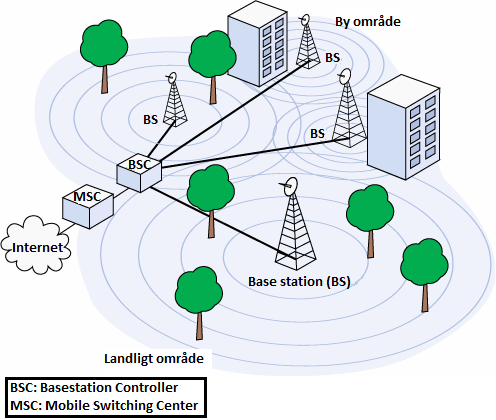
\includegraphics []{Billeder/celler.png}
\caption {Celler, som hver dækker deres eget geografiske område \cite{techviral}}
\label {celler}
\end{figure} 

Når man bruger sin mobiltelefon vil den, gennem luften, skabe kontakt til den nærmeste basestation, se figur \ref{GSM}. Hvis man har sendt en SMS-besked, vil denne modtages af basestationen, som sender den videre til SMS-centeret. SMS-centeret er herefter ansvarlig for at viderebringe SMS’en til modtageren. Hvis SMS-centeret ikke kan få forbindelse til modtagertelefonen (hvis denne er slukket eller udenfor signal), gemmes beskeden i centeret og sendes når der er oprettet forbindelse til modtageren. På figuren er der indtegnet et link mellem mobiltelefon og SMS-center, disse kaldes ”Mobile switching centre” og er netværksenheder, som tager sig af den trådløse kommunikation. \cite{info}

\begin{figure}[H]
\includegraphics []{Billeder/GSMnetværk.png}
\caption {SMS'ens vej fra afsender til modtager \cite{info}}
\label {GSM}
\end{figure} 

I GSM er der indbygget to muligheder for at sende en flere af SMS-beskeder sammen. Den ene mulighed er SMS-sammenkædning, hvilket vil sige at en række SMS-beskeder bliver kædet sammen og sendes hver for sig, men hos modtageren bliver de sat sammen i samme rækkefølge og læses igen som én besked. Den anden mulighed er komprimering af tekst med huffman coding.[active] Hvis denne mulighed udnyttes kan man sende optil 80 tegn mere pr. SMS besked. Dette kræver dog at telefonen fra fabrikkens side har sprogspecifik kompressions parametre. Dette kræver plads og langt de fleste mobiltelefonproducenter vælger, ifølge en artikel fra University of Teknology Sydney, skrevet af Kuross Amri og Tom Ceglearek, at bruge denne plads på spil og ringetoner \cite{UNI}. 


	\section{SMS teknologi}
	Langt de fleste mennesker beskæftiger sig dagligt med SMS'er - dog uden at vide hvad der i virkeligheden sker, når der sendes en SMS. Selv når en mobiltelefon ikke er i brug, sender og modtager den små datapakker til/fra SMS-centeret. Disse data hjælper blandt andet med at lokalisere de basestationer, mobiltelefonen er tættest på.

Når en SMS-besked bliver sendt fra en mobiltelefon, bliver den i første omgang sendt til mobilcentralen via basestationerne. Når mobilcentralen modtager beskeden bliver den overført til et SMS-center (SMSC). SMS-centeret tager sig af at sende beskeden til den rette modtager, ved at overføre den til den ønskede modtagers SMS-center. Når beskeden når frem til den pågældendes center, bliver den, hvis det er muligt, overført til mobilcentralen der sender beskeden til modtageren. SMS-centeret kan endvidere sende en bekræftelse til afsenderen, når beskeden bliver leveret til modtageren. Et overblik over kommunikationen ses i figur \ref{smsTransm}. Alt dette er muligt via Signaling System no. 7 - som er en protokol suite, der indeholder forskellige protokoller. Protokollerne benyttet af SMS-systemer, befinder sig mere specifikt i SS7 suitens Mobile Application Part (MAP). \cite{Pro_1} \cite{sms_max1}

\noindent
\begin{figure}[hba]
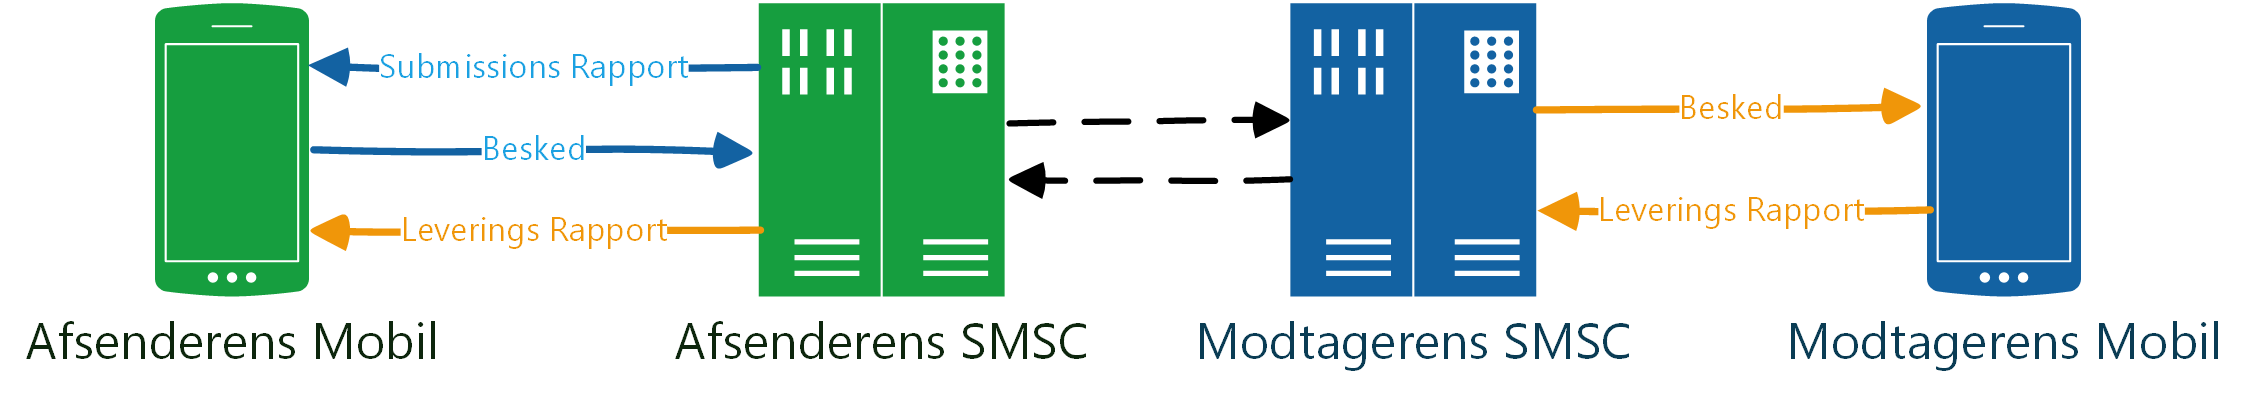
\includegraphics[width=\linewidth]{Billeder/Mobil.png}
\caption {Kommunikationen ved transmission af SMS-beskeder.}
\label{smsTransm}
\end{figure}

Signalerings systemerne i MAP er efter design begrænset til visse størrelser af data. Da man byggede SMS-systemet, talte man tegnene i forskellige beskeder, hvorefter man fandt ud af, at langt de fleste var under 160 tegn. Man mente derfor, at 160 tegn var rigeligt til at rumme de fleste beskeder, hvorved en SMS-beskeds maksimale størrelse blev derfor defineret til 160 tegn. Efter introduktion af udvidede tegnsæt er definitionen præciseret til 1120 bits (160 tegn * 7 bit). \cite{sms_max1} \cite{sms_max2}


Da begrænsningen er defineret i bits, er beskedens maksimale længde afhængig af det anvendte tegnsæt. Det mest almindelige tegnsæt er det grundlæggende 7-bit GSM alfabet. Dette alfabet benytter 7-bits til at symbolisere tegn, hvilket udgør 128 forskellige muligheder. 7-bit GSM alfabetet begrænser derfor en SMS-beskeds længde til 1120/7 bits = 160 tegn. Når der er brug for mere avancerede specialtegn, bruger SMS-systemer UCS-2 tegnsættet. Dette tegnsæt benytter 2 okteter - altså 16 bits - til repræsentation af ét tegn. Ved brug af dette tegnsæt mindskes den maksimale længde derfor ned til 1120/16 = 70 tegn. \cite{sms_pdu}

Enhver SMS-besked indeholder også en header\cite{sms_pdu}, som der er afsat plads til udover de 140 okteter. En SMS-header indeholder typisk data som f.eks. afsenderens telefonnummer, længden af beskeden, benyttet tegnsæt og lignende. Hvis en SMS-besked bliver længere end grænsen, på det benyttede tegnsæt, bliver beskeden delt op i flere beskeder. Når en besked bliver delt op, skrives der information til fletning af beskeden i headeren - og da der ikke er afsat plads til ekstra header information, bliver der brugt 6 okteter af de oprindelige 140 i beskeden. Dette begrænser længden yderligere til 153 ved 7-bit encoding og 67 ved 16-bit encoding. 

	
	\section{Tegnsæt}
	For at kunne komprimere en besked er det vigtigt at kende til teknologien bag sms’er.

Den teknologi som anvendes i moderne telefoner hedder GSM (Global System for Mobile Communications), som er en 2G standard.# Denne teknologi gør det muligt at benytte sig af sms’er.

For at et computersystem skal have muligheden for at kunne printe tegn til skærmen, er det nødvendig at repræsentere disse tegn med hver sit tal. Disse tal har man bestemt i en standard, som betyder at alle skal benytte de samme tal, for de samme tegn, og derved gøre det lettere for programmørerne af softwaren der benytter disse tegn. Den mest brugte standard indenfor tegnsæt, som dette kaldes, er unicode#

I mobiler der gør brug af GSM, kan der til sms’er, benyttes et tegnsæt kaldt GSM 03.38. Dette tegnsæt kan kodes i en række alfabeter, hvor standard alfabetet GSM 7 bit er et krav ved skabelse af mobiltelefoner.

Nedenunder ses et skema af GSM 7 bit alfabetet:
	
	\section{Komprimeringsalgoritmer}
	\subsection{Huffman coding}
Komprimeringsalgoritmen "Huffman coding", er udviklet af David A. Huffman. Huffman udviklede algoritmen, mens han var Ph.D studerende på MIT. I 1952 udgav han dokumentet"A Method for the Construction of Minimum-Redundancy Codes"\cite{A_Method_for}. Her beskrev Huffman, hvordan hans komprimerings algoritme fungerede. Hvad han havde udviklet, var en 'lossless' (tabsfri) komprimerings metode, hvilket betyder, at der ikke vil være noget tab af information ved at komprimere. Komprimeringsmetoden er beregnet til binære systemer, og formålet med algoritmen er at få en given datamænde til at benytte et minimalt antal bit. 

For så at kunne få de orginale data tilbage fra den komprimerede form, kræver det selvfølgelig, at man har en form for ordbog, der beskriver hvilke tegn, der hører sammen med hvilke bits.

For at Huffman coding effektivt kan fungere, skal algoritmen have adgang til hele datamængden, for at kunne analysere hyppigheden af forskellige tegn. Dette betyder at algoritmen skal løbe i gennem datamængden to gange. Første gang, for at indsamle statistik, og anden gang for så at foretage den reelle komprimering. En eksempel på en algoritme der ikke har den ulempe er komprimeringsmetoden "Lempel-Ziv-Welch".


\subsubsection{Generering af Huffman træ}
Huffman algoritmen kigger på frekvensen af tegn, og giver så de hyppigste tegn, den korteste binære kode. For at finde frem til de binære koder til hver tegn, laver man et huffman træ. Træet gør, at den binære kode til et tegn, aldrig vil være starten på koden til et andet tegn. Træet laves ved først at tælle hyppigheden af de forskellige tegn brugt i datamængden der skal komprimeres, og derefter tage de to tegn med lavest frekvens, og lave et nyt punkt, med frekvensen af det første og andet tegn lagt sammen. Dette gøres så indtil der kun er et punkt tilbage. Dette punkt er så toppen af træet. For så at finde frem til den binære kode for hvert tegn, starter man i toppen af træet, og tilføjer 0 eller 1, hvis man gå til henholdsvis venstre eller højre.
\\
\\
Hvis vi kigger på sætningen "dette er et eksempel", viser tabel \ref{tab:huffmantable_new} de forskellige tegn brugt i sætningen, sorteret efter hyppighed. Her tager vi så de to tegn med lavest frekvens (fx D og K), og laver et nyt punkt, med frekvensen af det første og andet tegn lagt sammen. Dette nye punkt, sættes så ind i listen, i stedet for de to tegn. Herefter laves der igen et punkt, med de to tegn/punkter med lavest frekvens, og dette gøres til der kun er et punkt tilbage. Det endelige resultat, bliver så Huffman træet, figur \ref{fig:huffmantree}. 



\begin{figure}[hba]
\centering
\begin{tabular}{|c|c|}
\hline
\cellcolor{ForestGreen}\color{white}{\textbf{Tegn}} &
\cellcolor{ForestGreen}\color{white}{\textbf{Frekvens}} \\ 
\hline 
E & 7 \\ 
\hline 
SPACE & 3 \\ 
\hline 
T & 3 \\ 
\hline 
R & 1 \\ 
\hline 
P & 1 \\ 
\hline 
S & 1 \\ 
\hline 
M & 1 \\ 
\hline 
L & 1 \\ 
\hline 
D & 1 \\ 
\hline 
K & 1 \\ 
\hline 
\end{tabular} 
\caption{Frekvens for tegn i sætningen ''dette er et eksempel''}
\label{tab:huffmantable_new}
\end{figure}

\begin{figure}[H]
\centering
%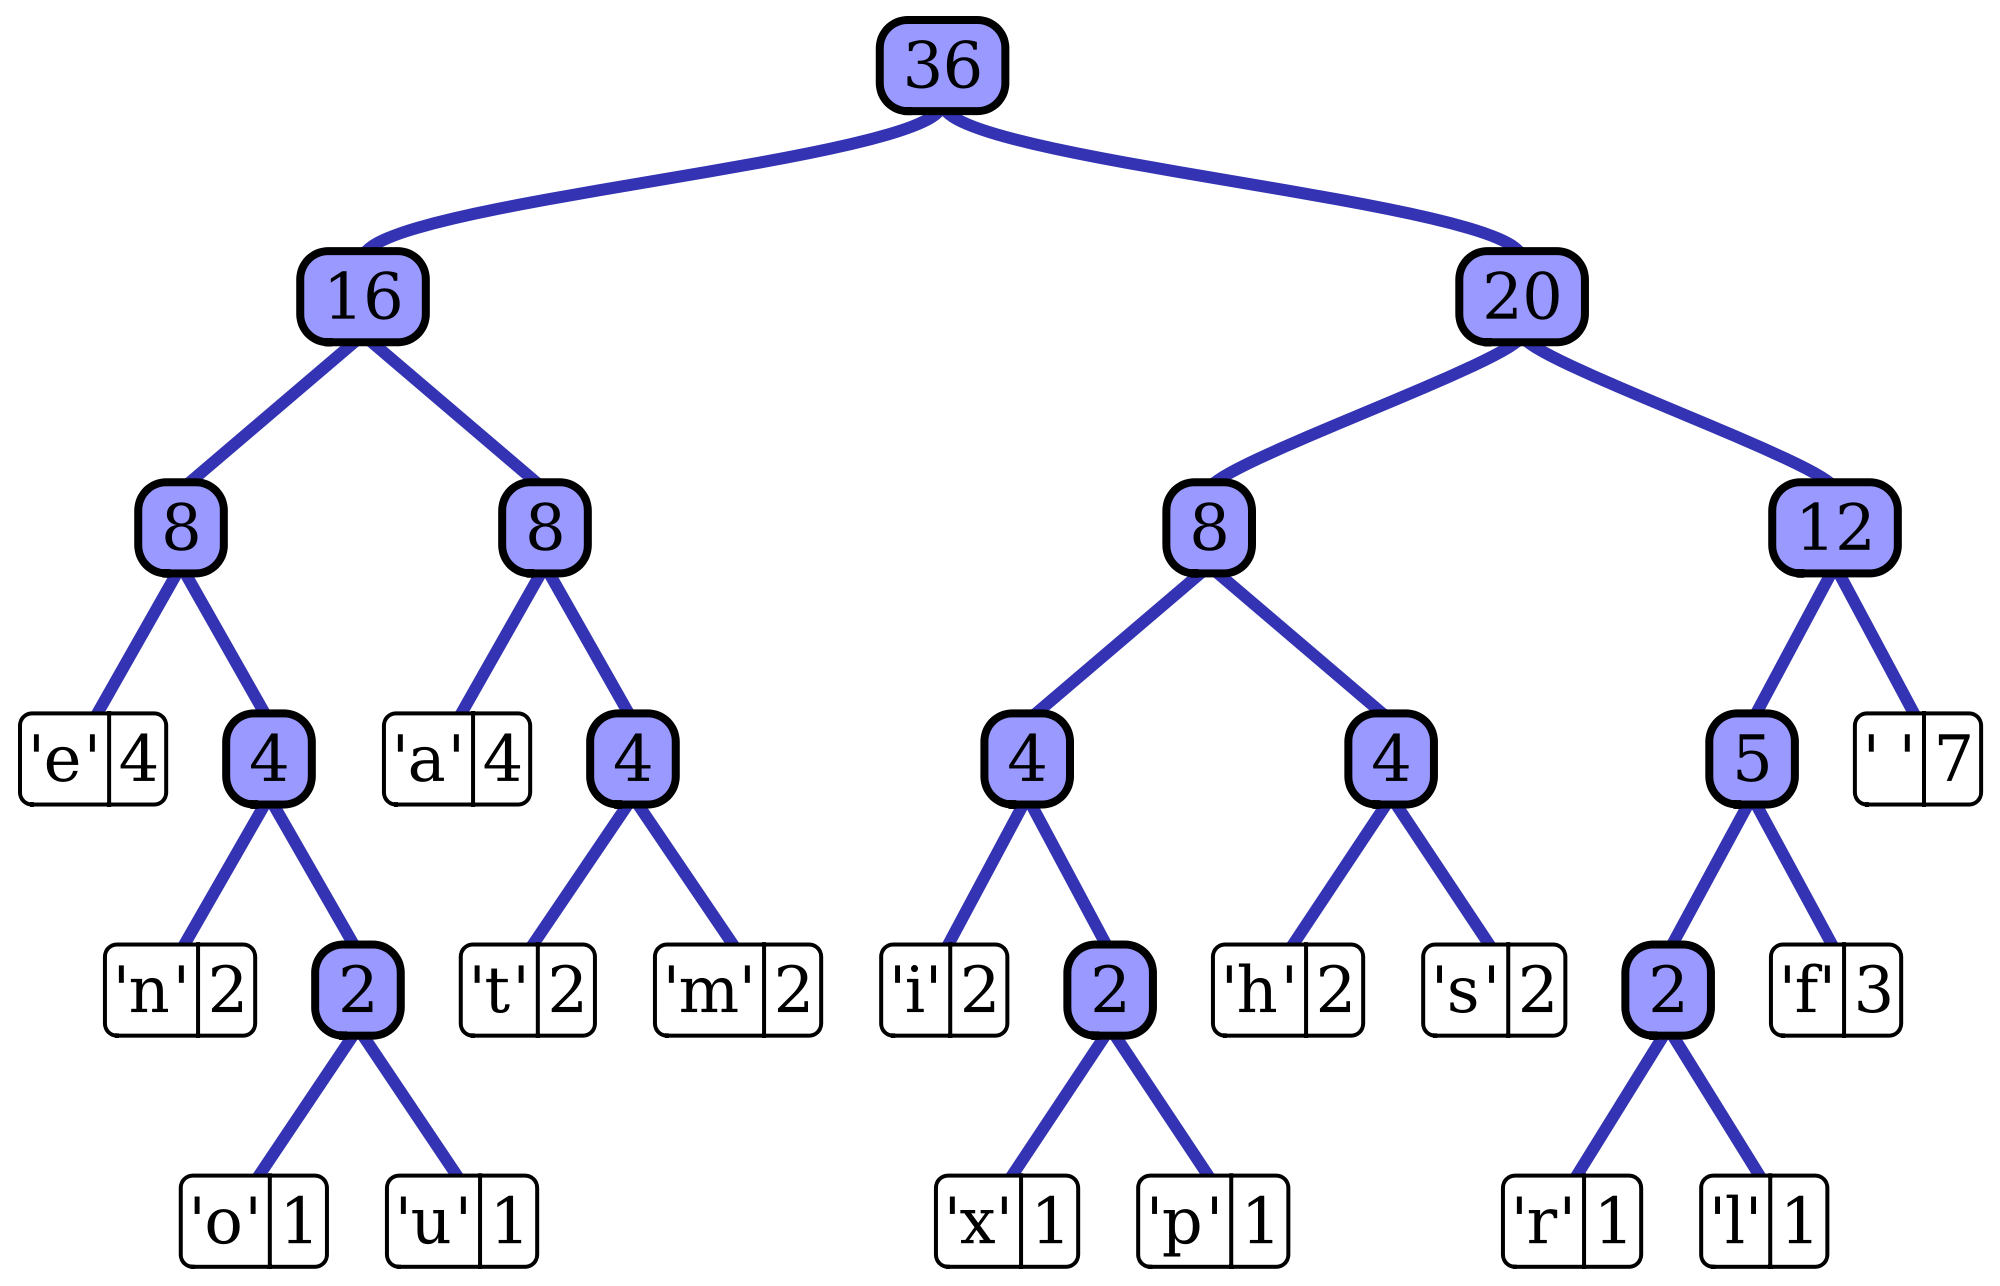
\includegraphics[width=\linewidth]{Billeder/Huffman_tree_2.png}
%

%

%

%
%
%

\enlargethispage{100cm}
% Start of code
% \begin{tikzpicture}[anchor=mid,>=latex',line join=bevel, scale=0.5]
\begin{tikzpicture}[>=latex',line join=bevel, scale=0.8]
  \pgfsetlinewidth{1bp}
%%
\pgfsetcolor{black}
  % Edge: ML -> L
  \draw [->] (271bp,85.689bp) .. controls (271bp,77.317bp) and (271bp,66.99bp)  .. (271bp,47.016bp);
  \definecolor{strokecol}{rgb}{0.0,0.0,0.0};
  \pgfsetstrokecolor{strokecol}
  \draw (274.5bp,64bp) node {1};
  % Edge: 2 -> S
  \draw [->] (127bp,85.689bp) .. controls (127bp,77.317bp) and (127bp,66.99bp)  .. (127bp,47.016bp);
  \draw (130.5bp,64bp) node {1};
  % Edge: 20 -> E
  \draw [->] (115.2bp,388.3bp) .. controls (112.76bp,381.27bp) and (109.84bp,372.85bp)  .. (103.66bp,355.07bp);
  \draw (116.5bp,372bp) node {0};
  % Edge: DK -> K
  \draw [->] (356.54bp,88.329bp) .. controls (365.3bp,78.844bp) and (377bp,66.163bp)  .. (394.43bp,47.282bp);
  \draw (388.5bp,64bp) node {1};
  % Edge: DK -> D
  \draw [->] (343bp,85.689bp) .. controls (343bp,77.317bp) and (343bp,66.99bp)  .. (343bp,47.016bp);
  \draw (346.5bp,64bp) node {0};
  % Edge: 2 -> P
  \draw [->] (113.46bp,88.329bp) .. controls (104.7bp,78.844bp) and (92.997bp,66.163bp)  .. (75.568bp,47.282bp);
  \draw (101.5bp,64bp) node {0};
  % Edge: 7 -> 4
  \draw [->] (213.57bp,242.43bp) .. controls (223.82bp,232.18bp) and (237.71bp,218.29bp)  .. (256.45bp,199.55bp);
  \draw (242.5bp,224bp) node {1};
  % Edge: 13 -> 6
  \draw [->] (158.9bp,315.02bp) .. controls (153.73bp,305.95bp) and (147.15bp,294.39bp)  .. (136.22bp,275.18bp);
  \draw (152.5bp,292bp) node {0};
  % Edge: 4 -> ML
  \draw [->] (271bp,165.69bp) .. controls (271bp,155.89bp) and (271bp,143.42bp)  .. (271bp,122.26bp);
  \draw (274.5bp,144bp) node {0};
  % Edge: 13 -> 7
  \draw [->] (175.19bp,314.3bp) .. controls (178.95bp,305.58bp) and (183.63bp,294.71bp)  .. (191.85bp,275.61bp);
  \draw (191.5bp,292bp) node {1};
  % Edge: 3 -> R
  \draw [->] (113.46bp,168.33bp) .. controls (104.7bp,158.84bp) and (92.997bp,146.16bp)  .. (75.568bp,127.28bp);
  \draw (101.5bp,144bp) node {0};
  % Edge: 6 -> 3
  \draw [->] (127bp,239.94bp) .. controls (127bp,231.81bp) and (127bp,221.88bp)  .. (127bp,202.44bp);
  \draw (130.5bp,224bp) node {0};
  % Edge: ML -> M
  \draw [->] (257.46bp,88.329bp) .. controls (248.7bp,78.844bp) and (237bp,66.163bp)  .. (219.57bp,47.282bp);
  \draw (244.5bp,64bp) node {0};
  % Edge: 20 -> 13
  \draw [->] (131.43bp,389.02bp) .. controls (137.45bp,379.79bp) and (145.16bp,367.99bp)  .. (157.6bp,348.93bp);
  \draw (150.5bp,372bp) node {1};
  % Edge: 3 -> 2
  \draw [->] (127bp,165.69bp) .. controls (127bp,155.89bp) and (127bp,143.42bp)  .. (127bp,122.26bp);
  \draw (130.5bp,144bp) node {1};
  % Edge: 6 -> SPACE
  \draw [->] (110.82bp,243.46bp) .. controls (100.85bp,235.1bp) and (87.659bp,224.06bp)  .. (67.583bp,207.26bp);
  \draw (100.5bp,224bp) node {1};
  % Edge: 7 -> T
  \draw [->] (199bp,239.94bp) .. controls (199bp,233.11bp) and (199bp,225.02bp)  .. (199bp,207.13bp);
  \draw (202.5bp,224bp) node {0};
  % Edge: 4 -> DK
  \draw [->] (284.54bp,168.33bp) .. controls (295.3bp,156.67bp) and (310.52bp,140.19bp)  .. (329.52bp,119.61bp);
  \draw (316.5bp,144bp) node {1};
  % Node: 2
\begin{scope}
  \definecolor{strokecol}{rgb}{0.0,0.0,0.0};
  \pgfsetstrokecolor{strokecol}
  \draw (127bp,104bp) ellipse (27bp and 18bp);
  \draw (127bp,104bp) node {2};
\end{scope}
  % Node: 13
\begin{scope}
  \definecolor{strokecol}{rgb}{0.0,0.0,0.0};
  \pgfsetstrokecolor{strokecol}
  \draw (168bp,332bp) ellipse (27bp and 18bp);
  \draw (168bp,332bp) node {13};
\end{scope}
  % Node: E
\begin{scope}
  \definecolor{strokecol}{rgb}{0.0,0.0,0.0};
  \pgfsetstrokecolor{strokecol}
  \draw (69bp,309bp) -- (69bp,355bp) -- (123bp,355bp) -- (123bp,309bp) -- cycle;
  \draw (97bp,332bp) -- (97bp,355bp);
  \draw (69bp,332bp) -- (123bp,332bp);
  \draw (83bp,337bp) node {E};
  \draw (110bp,337bp) node {7};
  \draw (96bp,314bp) node {0};
\end{scope}
  % Node: D
\begin{scope}
  \definecolor{strokecol}{rgb}{0.0,0.0,0.0};
  \pgfsetstrokecolor{strokecol}
  \draw (316bp,1bp) -- (316bp,47bp) -- (370bp,47bp) -- (370bp,1bp) -- cycle;
  \draw (344bp,24bp) -- (344bp,47bp);
  \draw (316bp,24bp) -- (370bp,24bp);
  \draw (330bp,29bp) node {D};
  \draw (357bp,29bp) node {1};
  \draw (343bp,6bp) node {11110};
\end{scope}
  % Node: SPACE
\begin{scope}
  \definecolor{strokecol}{rgb}{0.0,0.0,0.0};
  \pgfsetstrokecolor{strokecol}
  \draw (0bp,161bp) -- (0bp,207bp) -- (82bp,207bp) -- (82bp,161bp) -- cycle;
  \draw (59bp,184bp) -- (59bp,207bp);
  \draw (0bp,184bp) -- (82bp,184bp);
  \draw (30bp,189bp) node {SPACE};
  \draw (71bp,189bp) node {3};
  \draw (41bp,166bp) node {101};
\end{scope}
  % Node: ML
\begin{scope}
  \definecolor{strokecol}{rgb}{0.0,0.0,0.0};
  \pgfsetstrokecolor{strokecol}
  \draw (271bp,104bp) ellipse (27bp and 18bp);
  \draw (271bp,104bp) node {2};
\end{scope}
  % Node: K
\begin{scope}
  \definecolor{strokecol}{rgb}{0.0,0.0,0.0};
  \pgfsetstrokecolor{strokecol}
  \draw (388bp,1bp) -- (388bp,47bp) -- (442bp,47bp) -- (442bp,1bp) -- cycle;
  \draw (416bp,24bp) -- (416bp,47bp);
  \draw (388bp,24bp) -- (442bp,24bp);
  \draw (402bp,29bp) node {K};
  \draw (429bp,29bp) node {1};
  \draw (415bp,6bp) node {11111};
\end{scope}
  % Node: M
\begin{scope}
  \definecolor{strokecol}{rgb}{0.0,0.0,0.0};
  \pgfsetstrokecolor{strokecol}
  \draw (172bp,1bp) -- (172bp,47bp) -- (226bp,47bp) -- (226bp,1bp) -- cycle;
  \draw (202bp,24bp) -- (202bp,47bp);
  \draw (172bp,24bp) -- (226bp,24bp);
  \draw (187bp,29bp) node {M};
  \draw (214bp,29bp) node {1};
  \draw (199bp,6bp) node {11100};
\end{scope}
  % Node: L
\begin{scope}
  \definecolor{strokecol}{rgb}{0.0,0.0,0.0};
  \pgfsetstrokecolor{strokecol}
  \draw (244bp,1bp) -- (244bp,47bp) -- (298bp,47bp) -- (298bp,1bp) -- cycle;
  \draw (272bp,24bp) -- (272bp,47bp);
  \draw (244bp,24bp) -- (298bp,24bp);
  \draw (258bp,29bp) node {L};
  \draw (285bp,29bp) node {1};
  \draw (271bp,6bp) node {11101};
\end{scope}
  % Node: 3
\begin{scope}
  \definecolor{strokecol}{rgb}{0.0,0.0,0.0};
  \pgfsetstrokecolor{strokecol}
  \draw (127bp,184bp) ellipse (27bp and 18bp);
  \draw (127bp,184bp) node {3};
\end{scope}
  % Node: P
\begin{scope}
  \definecolor{strokecol}{rgb}{0.0,0.0,0.0};
  \pgfsetstrokecolor{strokecol}
  \draw (28bp,1bp) -- (28bp,47bp) -- (82bp,47bp) -- (82bp,1bp) -- cycle;
  \draw (55bp,24bp) -- (55bp,47bp);
  \draw (28bp,24bp) -- (82bp,24bp);
  \draw (42bp,29bp) node {P};
  \draw (69bp,29bp) node {1};
  \draw (55bp,6bp) node {10010};
\end{scope}
  % Node: S
\begin{scope}
  \definecolor{strokecol}{rgb}{0.0,0.0,0.0};
  \pgfsetstrokecolor{strokecol}
  \draw (100bp,1bp) -- (100bp,47bp) -- (154bp,47bp) -- (154bp,1bp) -- cycle;
  \draw (127bp,24bp) -- (127bp,47bp);
  \draw (100bp,24bp) -- (154bp,24bp);
  \draw (114bp,29bp) node {S};
  \draw (141bp,29bp) node {1};
  \draw (127bp,6bp) node {10011};
\end{scope}
  % Node: R
\begin{scope}
  \definecolor{strokecol}{rgb}{0.0,0.0,0.0};
  \pgfsetstrokecolor{strokecol}
  \draw (28bp,81bp) -- (28bp,127bp) -- (82bp,127bp) -- (82bp,81bp) -- cycle;
  \draw (56bp,104bp) -- (56bp,127bp);
  \draw (28bp,104bp) -- (82bp,104bp);
  \draw (42bp,109bp) node {R};
  \draw (69bp,109bp) node {1};
  \draw (55bp,86bp) node {1000};
\end{scope}
  % Node: T
\begin{scope}
  \definecolor{strokecol}{rgb}{0.0,0.0,0.0};
  \pgfsetstrokecolor{strokecol}
  \draw (172bp,161bp) -- (172bp,207bp) -- (226bp,207bp) -- (226bp,161bp) -- cycle;
  \draw (200bp,184bp) -- (200bp,207bp);
  \draw (172bp,184bp) -- (226bp,184bp);
  \draw (186bp,189bp) node {T};
  \draw (213bp,189bp) node {3};
  \draw (199bp,166bp) node {110};
\end{scope}
  % Node: 7
\begin{scope}
  \definecolor{strokecol}{rgb}{0.0,0.0,0.0};
  \pgfsetstrokecolor{strokecol}
  \draw (199bp,258bp) ellipse (27bp and 18bp);
  \draw (199bp,258bp) node {7};
\end{scope}
  % Node: 6
\begin{scope}
  \definecolor{strokecol}{rgb}{0.0,0.0,0.0};
  \pgfsetstrokecolor{strokecol}
  \draw (127bp,258bp) ellipse (27bp and 18bp);
  \draw (127bp,258bp) node {6};
\end{scope}
  % Node: 20
\begin{scope}
  \definecolor{strokecol}{rgb}{0.0,0.0,0.0};
  \pgfsetstrokecolor{strokecol}
  \draw (121bp,406bp) ellipse (27bp and 18bp);
  \draw (121bp,406bp) node {20};
\end{scope}
  % Node: 4
\begin{scope}
  \definecolor{strokecol}{rgb}{0.0,0.0,0.0};
  \pgfsetstrokecolor{strokecol}
  \draw (271bp,184bp) ellipse (27bp and 18bp);
  \draw (271bp,184bp) node {4};
\end{scope}
  % Node: DK
\begin{scope}
  \definecolor{strokecol}{rgb}{0.0,0.0,0.0};
  \pgfsetstrokecolor{strokecol}
  \draw (343bp,104bp) ellipse (27bp and 18bp);
  \draw (343bp,104bp) node {2};
\end{scope}
%
\end{tikzpicture}
% End of code

%



\caption{Huffman træ for sætningen ''dette er et eksempel''}
\label{fig:huffmantree}
\end{figure}


\subsection{Lempel-Ziv-Welch}
Lempel-Ziv-Welch
	
	\section{Problemdokumentation}
	N�r det kommer til SMS beskeder, s� er der en gr�nse p� hvor mange tegn der kan v�re i en enkelt besked. For det latinske alfabet ligger begr�nsningen p� 160 tegn. Begr�nsningen �ndrer sig fra tegns�t til tegns�t. For eksempel har det kinesiske alfabet en tegnbegr�nsning p� 70 tegn\cite{Pro_1}. Normalt vil en besked som fylder mere end sin tegnbegr�nsning blive delt op i to separate beskeder, hvis afsenderen af beskeden ikke selv g�r det, hvilket kommer til at betyde dobbelt SMS takst. Med denne begr�nsning i tankerne kommer sp�rgsm�let: Hvor betydeligt er dette problem, og er det overhovedet v�rd at kigge n�rmere p�?
Erhvervs priserne for at sende en SMS inden for Norden og Eurozonen er betydeligt billigere end hvis man sendte til eller fra et Europa land ikke inde under EU, og n�r man sender til eller fra lande udenfor Europa s� bliver det kun dyrere og dyrere. Et internationalt firma som udnytter SMS til intern kommunikation eller andet kan ende med at bruge mange penge p� deres telefonregninger. Tilbage i 2009/2010 begyndte de forskellige telefonselskaber at h�ve prisen p� afsendelse af beskeder til udlandet. TDC's pris, for eksempel, gik fra at v�re p� 2,40 kr. til at koste 3,20 kr. per SMS\cite{Pro_2}. Nedenst�ende tabel viser Telenors SMS takst samt minutpris for erhverv ved at sende beskeder til Danmark, men prisen er stadig den sammen den fra Danmark til udlandet\cite{Pro_3}.

%\noindent
\begin{table}[H]
\begin{center}
\begin{tabular}{ | l | r |}
    \hline
    \cellcolor{ForestGreen} &  \cellcolor{ForestGreen}\color{white}{\textbf{Sende/Modtage SMS}}\\[2ex] \hline
    \textbf{Norden} & 0,66 kr./sms \\ \hline
    \textbf{EU} & 0,66 kr./sms \\ \hline
    \textbf{�vrige Europa} & 3,20 kr./sms \\ \hline
    \textbf{Verden 1} & 3,20 kr./sms \\ \hline
    \textbf{Verden 2} & 3,20 kr./sms \\ \hline
    \textbf{Skibe m. MCP-d�kning} & 3,20 kr./sms \\ \hline
\end{tabular} 
\caption{Tabel over SMS-Priser fra Telenor ~\cite{Pro_3}}
\end{center}
\end{table}

Ligeledes er priserne for private hen over landegr�nserne heller ikke noget at prale af. I det private str�kker priserne sig fra 3's pris pr. SMS p� 2,50 kr\cite{Pro_4} til Telia's pris pr. SMS p� 4,00 kr\cite{Pro_5}. Uanset om man er privat eller erhvervsdrivende s� vil man gerne v�re sparsomme med antallet af beskeder man sender over landegr�nserne, og derudfra g�re god brug af sine 160 tegn s�dan at man undg�r dobbelt SMS takst ved at beskeden bliver delt i to.
Statistikkerne viser at der i 2011 blev sent omkring 12 milliarder SMS?er i Danmark alene, et fald fra forrige �r som l� p� 13 millarder, men det viser at der stadigv�k er h�jst forbrug af SMS beskeder. Derudover s� steg den mobile datatrafik fra 15 milliarder MB i 2010 til 26 milliarder MB i 2011\cite{Pro_6}. En l�sning som komprimere beskeder kunne ogs� hj�lpe til at d�mpe belastningen p� det mobile datatrafik netv�rk.
Derfor vil en eller anden datalogisk l�sning, som g�r det lettere at sende beskede, uden at man skal bekymre som om hvorvidt ens besked har mere end de begr�nsede 160 tegn, v�re aktuelt. S�dan en l�sning kan b�de g�re det mere bekvemt for brugeren at bruge SMS'er, og i det lange l�b sparer brugeren penge.
	
	\section{Interessenter}
	I forbindelse med projektet er der blevet tænkt over en række metoder, som gør os i stand til at finde ind til vores problems kerne, og understøtte problemet i sin helhed.
Ud fra projektforslaget er det blevet fastsat at vores endelige løsning til problemet skal være en prototype af et program. Denne prototype skal være skrevet i C, men da problemstillingen omhandler SMS-beskeder, er det  SMS-mediets krav, som vi skal designe vores løsning efter.


Ud fra vores problem findes der en række interessenter, som påvirkes af denne problemstilling.
På den følgende brainstorm, ses hvordan disse interessenter fordeler sig, ud fra det initierende problem, og hvordan de forbindes til hinanden.

\begin{figure}[H]
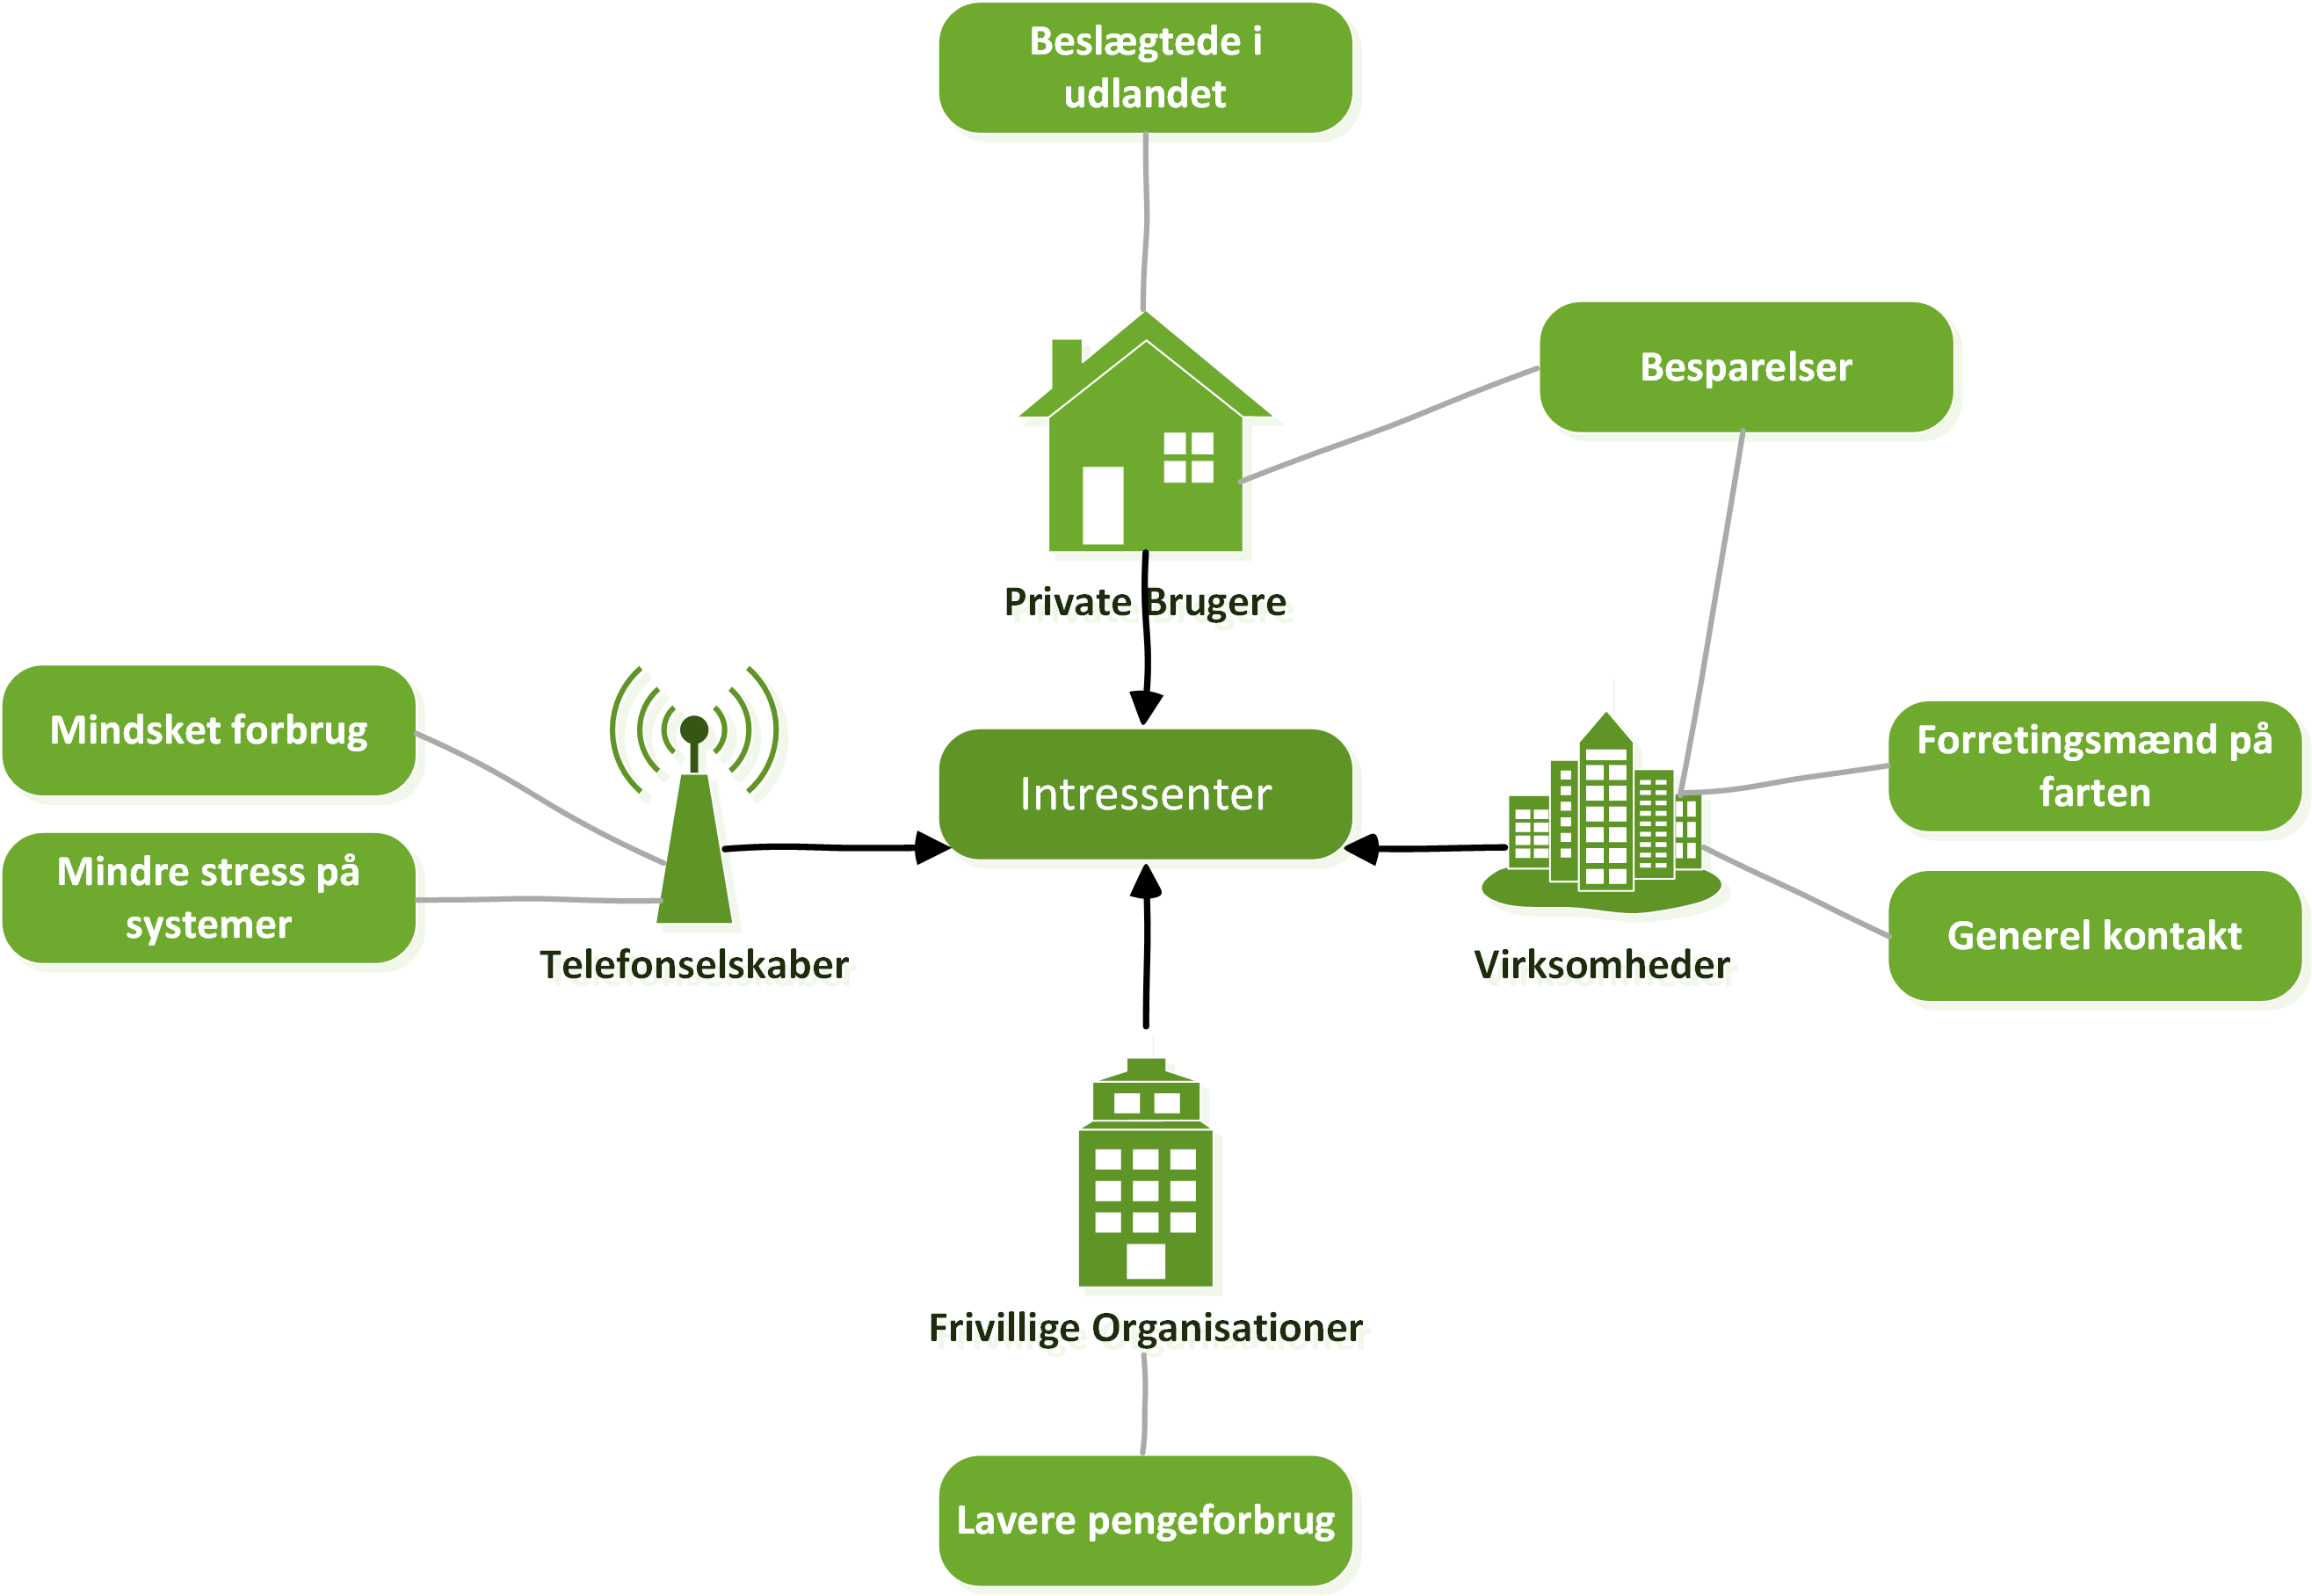
\includegraphics[width=\linewidth]{Billeder/Brainstormting.png}
\caption{Her ses hvordan interessenterne fordeler sig.}
\end{figure}

Denne brainstorm identificerer vores primære interessenter, som vil være vores hovedmålgruppe.
Man kan dele interessenterne ind i nogle grupper, henholdsvis: Private personer, internationale firmaer, frivillige organisationer og teleselskaber.
Hver af disse grupper har sin egen grund til at være interesseret i vores problemstilling, og derfor kan det også betyde, at der skal forskellige løsninger til at kunne løse problemstillingen, for hver forskellig interessent.


Ud fra vores problemstilling findes der en række data som kan være anvendelig i forhold til undersøgelsen af de førnævnte interessenter.


Viden om brugen af SMS'er hos de forskellige interessent grupper.
Det er vigtigt at finde ud af hvordan de forskellige interessenter bruger SMS'er som et medie. Med dette menes både hvor tit det bruges, men også i hvilken forbindelse og med hvem kommunikationen foregår.


Til indsamling af data omkring disse interessenter er det nødvendigt at komme i direkte kontakt med den målgruppe vi har med at gøre. Dette betyder at vi bliver nødt til at benytte nogle metoder, som gør det muligt at indsamle eller observere målgruppens forbrug af SMS'er.
Til dette vil en spørgeskema undersøgelse være velegnet, da brugen af SMS'er er data velegnet til kvantitative undersøgelser, da det er et spørgsmål om hvor mange SMS'er der sendes.


	\section{Eksisterende løsninger}
	Der findes flere forskellige former for programmer der allerede helt eller delvist l�ser sms- begr�nsnings problemet. Vi vil i det f�lgende afsnit tage udgangspunkt i to eksisterende programmer.

Det f�rste program hedder SMS ZIP og virker kun til smartphones med Windows som operativsystem. Dette program er af typen ikke tabsfri, da det g�r ind og fjerner alle un�dige mellemrum i teksten, og erstatter f�rste bogstav i f�lgende ord med et stort bogstav, s�ledes at teksten stadig kan l�ses. Ydermere er det programmeret til at kunne identificere bestemte ord og s� erstatte disse med forkortelser. Programmet er indrettet s�ledes at brugeren selv skal v�lge om hver enkelt besked skal komprimeres. Et eksempel p� hvordan programmet vil komprimere en besked:\cite{download-sms} 
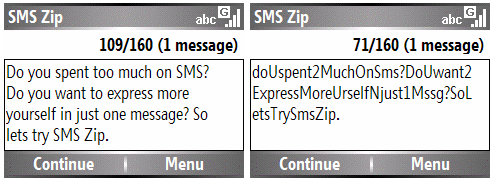
\includegraphics []{Billeder/SMSZIP.png}

Denne konkrete besked bliver alts� kortet ned fra 109- til 71 tegn. En af fordelene ved dette program er at modtageren ikke beh�ver et tilsvarende dekomprimeringsprogram for at kunne l�se beskeden. En anden fordel er at beskeder der ikke overg�r en begr�nsningen, ikke n�dvendigvis bliver komprimeret. Denne l�sning har dog en del flere ulemper end fordele. Den �benlyse ulempe er at beskederne bliver en hel del sv�rere at l�se, og kan v�re en mulig irritation for mange, n�r de l�ser beskeden. En anden klar ulempe er at der bliver brugt en del slang for at g�re ordene kortere, slang s�som tallet ?2? i stedet for ordet ?to?. Dette kan bevirke at budskabet er sv�rere at tage seri�st. Yderligere er det et problem at programmet kun virker til windowsphones og at forkortelserne kun er beregnet til engelsktalende beskeder. Det er derfor, p� baggrund af ovenst�ende, vores vurdering at programmet er en ufuldst�ndig l�sning, og er derfor ikke tilstr�kkelig.\cite{download-sms}

En anden eksisterende l�sning hedder SMS ZIPPER. Det er p� mange punkter et totalt modstridende program i forhold til SMS ZIP. F�rst og fremmest er det forskelligt da dette er et tabsfrit komprimerings program. Programmet virker p� langt de fleste smartphones og er, i mods�tning til SMS ZIP, en l�sning der komprimerer beskeden hos afsenderen og derefter dekomprimerer beskeden igen hos modtageren. Dette kr�ver dog at b�de afsender og modtager har programmet installeret. Programmet starter p� modtagerens telefon liges� snart en komprimeret besked modtages, s� beskeden kan l�ses med det samme uden besv�r for l�seren. Producenten lover helt op til 480 tegn pr. besked, alts� 3 gange s� mange tegn som en almindelig sms. Derudover fungerer programmet til flere sprog, heriblandt dansk, engelsk og tysk.\cite{smszipper} 

Dette program bruger en fleksibel algoritme til at komprimere beskederne. De har designet algoritmen direkte med henblik p� s�kaldte korte beskeder, alts� beskeder omkring de 160 tegn. Endvidere bruger programmet ogs� andre kodnings modeller, som kan v�re beregnet specifikt p� bestemte sprog eller typer af beskeder.

Vi har i ovenst�ende afsnit valgt at tage to vidt forskellige programmer under luppen, for at tegne en kontrast mellem en meget simpel og en mere avanceret l�sning. Vi ser at de hver is�r har deres fordele og ulemper, og disse vil vi tage til overvejelse i vores program.

	\section{Afgrænsning}
	Dette afsnit kommer omkring nogen af de valg, der blev lavet for at indskrænke projektets problemfelt. For det første er der forskellige tjenester og teknologier, som giver muglihed for at sende en kort besked, men med et begrænset antal tegn pr. besked. Eksempelvis er der SMS-beskeder med en begrænsning på 160 tegn når man bruger tegn fra tegnsættet GSM 7-bit\cite{Pro_1} og der er også internettjenester som for eksempel Twitter, som har en tegnbegrænsning på 140 tegn\cite{pro_af1}. Twitters formål har fra starten af, været at give mulighed for at sende korte og smertefrie bidder af information over internettet, og ikke lange blogs og artikler. Denne holdning er folkene bag Twitter meget konsekvente med\cite{pro_af2}. Derudover så er det også gratis at gøre brug af Twitter og derfor er det ikke ligeså væsentligt som SMS, som koster penge. Derfor har vi valgt ikke at arbejde med Twitter. Istedet vil projektet blive begrænset til at handle om SMS-beskeder.

Nu hvor valget om SMS eller Twitter er på plads, så kommer spørgsmålet om hvorvidt der skal arbejdes med smartphones eller almindelige mobiltelefoner. Smartphones har den fordel, at de kan implementere applikation uden alt for meget besvær, hvorimod på almindelige telefoner er det mere besværligt at installere programmer. Statistikkerne viser at flere og flere begynder at få smartphones\cite{pro_af3}. I det sidste kvartal af 2011 blev der solgt over 37 millioner iPhones, Apple's smartphone, i hele verdenen, som er højere end antallet af børn født i den samme periode\cite{pro_af4}. Derudover så bliver der også vist, at brugen af hjemme computere er dallende i det, at adgang til internettet også er tilgængeligt gennem smartphones, som derved gør det muligt for en person at være på internettet hvor man ellers ikke ville have tilgang til en almindelig computer\cite{pro_af3}. Dette kan betyde, at flere personer bruger SMS, fordi de bruger deres mobile enheder mere. Dog kan det også betyde at flere mennesker bruger e-mail i stedet for SMS fordi de alligevel har adgang til internettet. Ud fra dette vil projektet yderligere blive begrænset, til ikke at prøve at implementere programmet på almindelige mobiltelefoner. Derudover så er det også vanskeligt, at implementere en applikation skrevet i C, som er et krav for dette projekt, på en smartphone. Derfor vil løsningen være en prototype, som kan fungere på en computer. 

Når løsningen skal laves, er der brug for en komprimeringsalgoritme. Tidligere er et par komprimeringsalgoritmer blevet gennemgået, for eksempel Huffman eller PPM, som kan bruges til at udvikle løsningen. PPM løsninger har det med at være de bedste til komprimering af tekst. Ligeledes er komprimeringskraften ved Huffman for sig selv også meget kraftig, men er ikke altid optimal. Det er muligt at bygge ovenpå en Huffman komprimeringsalgoritme med PPM. PPM har dog et behov for en del mere RAM i forhold til Huffman, for at kunne komprimere, og er også en langt mere kompliceret løsning at udvikle. Ud fra projektets rammer samt den teoretiske platform som løsningen skulle kunne køre på, en mobiltelefon, så er Huffman løsningen den bedste mulighed. Derfor vil løsningen blive indskrænket til at bruge Huffman som komprimeringsalgoritme.\cite{pro_af5}

Løsningen skal kunne køre uden at forstyrre brugeren af programmet alt for meget. Her gælder blandt andet den tid det tager for programmet at komprimere beskeden, samt hvor meget plads og regnekraft det tager. Det er blandt andet derfor, at det blev besluttet løsningen skulle udvikles ud fra Huffman alene, og ikke lave løsningen med PPM. Ligeledes så skal det heller ikke være nødvendigt for brugeren selv at gøre noget for at komprimere beskeden. Komprimering skal ske automatisk i SMS-processen, uden at brugeren behøver at sætte det igang. Hvis det er nødvendigt med yderlig bruger interaktion, så skal det foregå så brugervenligt som muligt.

Det sidste punkt er hvilke tegnsæt som løsningen skal være i stand til at komprimere og dekomprimere. Skal tegn fra det kyrilliske alfabet eller specialtegn som Æ, Ø, Å og ß være i stand til at blive komprimeret, for eksempel. Det er blevet bestemt, at løsningen skal have implementeret GSM 7-bit tegnsættet, som er standard tegnsættet til SMS-beskeder på mobiltelefoner og smartphone.

	\section{Problemformulering}
	Ud fra vores problemanalyse har vi fundet ud af, at der klart er penge at spare, hvis man fra udlandet kan sende én besked i stedet for to. Vi har ligeledes set på eksisterende løsninger som SMS ZIP, for at undgå at lave de fejl, vi mener der er ved de programmer. Derudfra skal vores løsning være mere implementeret, således at brugeren aldrig kommer til at beskæftige sig med den komprimerede besked, så komprimering og dekomprimering sker automatisk. Vi er på baggrund af dette kommet frem til følgende problemformulering:

\begin{itemize}
\item[] \emph{Hvordan kan man spare forbrugeren for dobbelt SMS-takst, ved brug af et komprimeringsprogram? Hvordan kan man undgå at programmet bliver en belastning for brugeren?}
\end{itemize}

Der vil arbejdes frem mod en prototype, der kan komprimere en kort besked, for siden at dekomprimere den på en anden enhed. 	
	
	\section{Produktkrav}
	Til dette projekt skal der udarbejdes en løsning i form at et program, som kan komprimere en kort tekstbesked. Komprimeringen vil gøre tekstbeskeden mindre, det vil sige beskeden fylder færre bytes, og skulle gerne både gøre det hurtigere at sende beskeden, fordi den er mindre, men også gøre det muligt at sende en besked over en bestemt tegn begrænsning, som f. eks. de begrænsede 160 tegn ved brug af det latinske alfabet i en SMS. Beskeden skal derefter dekomprimeres hos modtageren, og derefter vise beskeden, som den så ud før den blev komprimeret. Denne proces skal ske, uden brugeren selv tager en direkte del i processen.

\begin {itemize}
\item Funktionelle Krav
\subitem Skal både være i stand til at komprimere og dekomprimere automatisk.
\subitem Programmet skal være i stand til at skelne mellem hvorvidt den pågældende besked skal komprimeres eller dekomprimeres.
\subitem Det er ikke forventet, at prototypen skal kunne køre på en mobil enhed som f. eks. en smartphone, men det er forventet at programmet kan bruges på en computer.

\item Ikke Funktionelle Krav
\subitem Produktet skal afleveres sammen med den tilhørende rapport, og har en fælles deadline den 19 december 2012.
\subitem Programmet skal skrives i programmeringssproget C.

\item Løsningsmål
\subitem Brugeren skal kunne gøre brug af programmet uden selv at tage direkte del i komprimerings-processen.
\subitem Programmet skal køre lokalt, og ligeledes skal komprimeringen og dekomprimeringen også ske lokalt.
\subitem Programmet skal implementeres og være brugbart.
\end{itemize}

	
%\chapter{Teori om komprimering?}



\chapter{Løsning}

  I dette kapitel beskrives løsningen på problemformuleringen. Kapitlet begynder med en mere dybdegående beskrivelse af den anvendte komprimeringsalgoritme og herefter beskrives dennes implementeringen. Slutteligt findes en mere reel beskrivelse af programmet, som danner løsning for projektet. 

	\section{Huffman træer}
	\label{huffman_traer}
	Hvis man vil komprimere en datamængde ved brug af huffmancoding, kræver det, at der bliver lavet et huffman træ. Dette træ kan genereres på tre forskellige måder: Statisk, dynamisk eller adaptivt. Principielt ser det resulterende bit-træ ens ud for hver af metoderne. Det handler mere om hvordan træerne bliver generet. I dette afsnit vil der være en gennemgang af hvordan disse metoder virker, samt deres fordele og ulemper i forhold til SMS beskeder. Den følgende tabel samt det følgende billede viser hvordan et potentielt Huffman bit-træ kunne se ud.

\begin{table}[H]
\begin{center}
\begin{tabular}{|c|c|}
    \hline
    \cellcolor{ForestGreen}\color{white}{\textbf{Tegn}}& \cellcolor{ForestGreen}\color{white}{\textbf{Forekomster}}\\[2ex] \hline
    A & 24 \\ \hline
    B & 12 \\ \hline
    C & 10 \\ \hline
    D & 8 \\ \hline
    E & 8 \\ \hline
\end{tabular} 
\caption{Et sæt tegn og forekomster. Hentet fra binaryessence.com}
\end{center}
\end{table}

\begin{figure}[H]
\centering
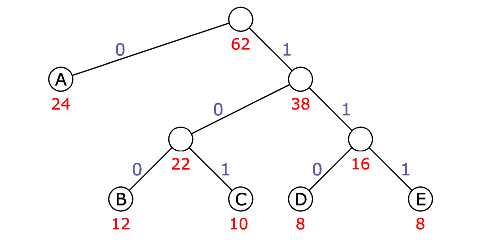
\includegraphics[width=\linewidth]{Billeder/huffman_tree.png}
\caption{Det samme sæt som før set i et Huffman træ. Hentet fra binaryessence.com}
\label{fig:huffmantree_fred}
\end{figure}

Ud fra billedet kan man se at de tegn som forekommer mindst er placeret nederst i træet, D og E, mens det tegn som forekommer mest er placeret øverst, A. Hver gang man går et niveau ned så går længden på et tegn op. A har en længde på 1 bit mens B, C, D og E har en længde på 3 bit. Tegnet som forekommer mest får altså den mindste længde. Derudover kan man også ud fra billedet se det følgende binære talsystem:

\begin{table}[H]
\begin{center}
\begin{tabular}{|c|c|c|}
    \hline
    \cellcolor{ForestGreen}\color{white}{\textbf{Tegn}} & \cellcolor{ForestGreen}\color{white}{\textbf{Binær Kode}} & \cellcolor{ForestGreen}\color{white}{\textbf{Kode Længde}}\\[2ex] \hline
    A & 0 & 1 \\ \hline
    B & 100 & 3 \\ \hline
    C & 101 & 3 \\ \hline
    D & 110 & 3 \\ \hline
    E & 111 & 3 \\ \hline
\end{tabular} 
\caption{Binært talsystem fra et Huffman træ. Hentet fra binaryessence.com}
\end{center}
\end{table}

Dette sæt af tegn og forekomster fylder i alt 496 bit for sig selv hvis man går ud fra hvert tegn fylder 1 byte, altså 8 bit. I et Huffman træ som dette billedet viser, fylder de samme tegn 138 bit som kan findes ved at lægge tegnene sammen i forhold til deres forekomster og længder. På billedet kan man også se punkter som ikke indeholder nogen tegn. Disse punkter kaldes for knuder og har en størrelse magen til summen af punkterne nedenunder den. Den øverste knude hvor træet altid starter kaldes for roden. Enderne på træet som indeholder de egentlige tegn kaldes for blade.\cite{Hufftree_1}

\subsection{Statisk}
Den første metode man kan bruge til at generere et Huffman træ, er den statiske metode. Et statisk Huffman træ bliver lavet ud fra formodede forekomster på i et stykke tekst. For eksempel hvis man kigger generelt på det engelske sprog, så forekommer tegnet ’e’ mest, og vil derfor blive placeret øverst i det statiske Huffman træ, mens tegn som ’z’ og ’x’ vil blive placeret nederst. Den statisk opbygning af et Huffman træ er standard metoden\cite{Hufftree_2}.

Et statisk Huffman træ virker på alle stykker tekst, især længere stykker af tekst som for eksempel artikler. Til gengæld kan den ende med at ikke gøre fuld brug af komprimeringskraften ved Huffman coding, når det handler om mindre beskeder, fordi det ikke altid går op med normalen for tegn forekomster i et sprog. Statiske Huffman træer virker bedre, i takt med at den tekst som skal komprimeres bliver større, og bliver mere ineffektiv, når teksten bliver mindre. Det er ikke sandsynligt, at den komprimerede tekst vil fylde mere, end hvis den ikke var komprimeret idet at Huffman komprimering er så effektivt som det er. \cite{Hufftree_3}

Fordele ved et statisk træ er at det let kan give gode resultater for større stykker af tekst og behøver ikke at sende noget yderligt i beskeden udover bitmønstret. Et statisk træ er også hurtigt idet at der ikke er behov for at generer et nyt træ for hvert eneste stykke tekst, som der er behov for med de to kommende metoder. Statisk kan derfor have en fordel fordi den ikke behøver ligeså meget regnekraft på enheder som mobiltelefoner, som muligvis kan være begrænset på det område.


\subsection{Dynamisk}
Den anden metode man kan bruge kaldes for et dynamisk Huffman træ. Et dynamisk træ bliver generet ud fra det reelle data som teksten består af. Træet bliver genereret ud fra den specifikke besked og er ikke en generel liste som ved den statiske metode. Det dynamiske træ er derfor den mest optimale til Huffman coding. Den dynamiske opbygning af et træ starter med at sætte de to tegn med færrest forekomster til en knude. Derefter bliver der bygget ovenpå den knude og tager hele tiden de tegn med færrest forekomster som endnu ikke er blevet sat ind i træet. En ny knude bliver lavet som får sat det næste tegn samt den foregående knude som indeholder alle tidligere tegn og knuder på.

\begin{figure}[H]
\centering
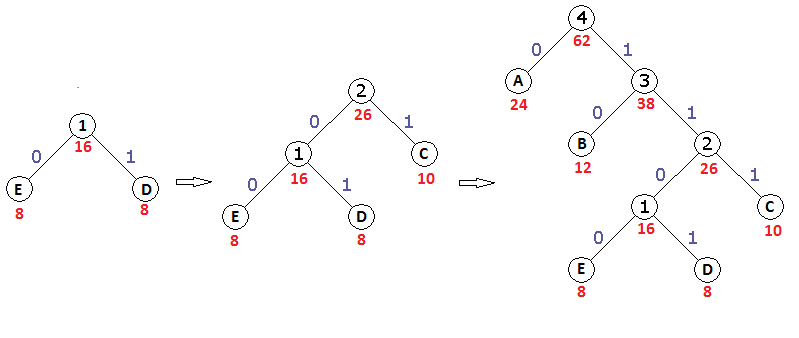
\includegraphics[width=\linewidth]{Billeder/dynamisk.png}
\caption{Dynamisk opbygning af et Huffman træ udfra det tidligere eksempel}
\label{fig:dynamic_tree}
\end{figure}

En ulempe ved den dynamiske metode er, at for at kunne dekode den komprimeret tekst  skal man bruge en kode tabel over træet. Idet at det er et træ skræddersyet til et bestemt stykke tekst, så har dem der skal dekode teksten ingen mulighed til hvordan man oversætter 0 og 1 tallene tilbage til den oprindelige tekst. Derfor er det nødvendigt med den dynamiske metode at medsende en tabel som angiver hvilke tegn har hvilke bitmønstre. Dette betyder selvfølgelig at den komprimeret tekst fylder et stykke mere og gør derfor ikke optimalt brug af komprimerings kraften ved Huffman coding. \cite{Hufftree_4}

Fordelen ved et dynamisk træ i forhold til det statiske er at den mere konstant gør optimal brug af Huffman coding til at komprimere et stykke tekst. Det er selvfølgelig det man gerne vil opnå i forhold til SMS beskeder, men som sagt så er det nødvendigt at sende en tabel med så det er muligt at dekode det komprimeret stykke tekst. Dette betyder at SMS beskeden fylder mere end hvis det bare var det komprimeret stykke tekst, og arbejder derfor imod målet om at formindske størrelsen af den data der bliver sendt.

\subsection{Adaptivt}
Den tredje og sidste metode til at komprimere et stykke tekst med Huffman coding er den adaptive metode. Med den adaptive metode starter træet med at intialisere forekomsten af tegn som de kommer til 1. Når det samme tegn fremkommer igen så vil det blive lagt til tegnets fremkomst værdi, og træet vil derefter også opdatere sig selv sådan hvis et nyt tegn begynder at have flest forekomster så vil den blive placeret øverst i træet.
I forhold til den foregående metode så kan den adaptive metode genere et træ alt efter hvad for noget data som skal komprimeres, ligesom den dynamiske metode, men har til gengæld ikke behov for at videregive en tabel som viser hvordan man oversætter det komprimerede tekst, idet at det adaptive træ på den enhed som dekomprimere vil gøre arbejdet og opdatere sig selv med det data den dekomprimere. Dette kan også betyde at det dynamiske træ muligvis ikke behøver at sende en tabel med over hvis dekomprimeringen sker ved hjælp af det adaptive træ. Ulempen ved den adaptive metode er at det stykke tekst der bliver komprimeret eller dekomprimeret ikke indgår i den nuværende version af træet, idet at det adaptive træ først opdateres med data fra tekststykket efter det er blevet komprimeret eller dekomprimeret. Derudover så kræver den også meget regnekraft fra den enhed som skal komprimere og dekomprimere fordi den konstant skal opdateres af det data den gennemarbejder. \cite{Hufftree_5}
I forhold til SMS beskeder så er den adaptive metoder sikkert bedst når det kommer til at formindske den mængde data der bliver sendt med beskeden. Ulempen er dog at træet har brug for tid til at komme op og køre ved at konstant opdatering af sit eget træ. Den adaptive metode starter derfor ud med at være langsom og ineffektivt idet at den introducere alle tegn fra bunden af og kan først effektivt komprimere efter den har arbejdet sig igennem et antal tekststykker. Kravet for regnekraft på enhederne der komprimere og dekomprimere  kan også være en større ulempe på en mobiltelefon.

\subsection{Sammenligning}
Alle tre modeller har sine fordele og ulemper. I dette afsnit der blive delkonkluderet på hele af afsnittet, og hver model vil blive sammenlignet med hinanden, og til resten af projektet, for at finde den model som bedst kan bruges til at besvare problemformuleringen omkring SMS beskeder.

Først er der den statiske model. Som sagt, så kræver den statiske model ikke særlig meget regnekraft. Derudover så er den også let at implementere fordi det er, som navnet hentyder, et statisk træ og er derfor altid ens. Ulempen ved den statiske model er at den ikke altid kan gøre optimalt brug af Huffman coding. Den tekst der skal komprimeres stemmer ikke altid overens med forekomst ratioen og kan derfor ikke gøre perfekt brug af Huffman. På dette punkt er både den dynamiske og den adaptive model bedre som kan lave sine egne træer alt efter hvad der skal komprimeres.

Med det kommer den dynamiske model. Af de tre modeller gør den dynamiske model bedst brug af komprimeringskraften ved Huffman coding idet at den laver et helt nyt træ ud fra det tekststykke den skal komprimere. Den dynamiske model har dog en del implementerings ulemper. Som sagt, så skal der sendes en manual med, som optager plads, for at kunne dekomprimere tekststykket igen. Derudover så kræver den dynamiske model også en del ekstra regnekraft på enheden for at generer et nyt træ hver gang der skal sendes en besked.

Den sidste model er den adaptive model. Fordelen ved den adaptive model er at den gør god brug af Huffman coding som den dynamiske model, og behøver ikke at sende noget ekstra med for at sikre modtageren kan dekomprimere beskeden, som den statiske model.Ulempen ved den adaptive model er at den ikke altid kan gøre optimalt brug af Huffman coding idet at træet først opdateres efter den har komprimeret og dekomprimeret et tekststykke. Derudover så er det også den model som kræver mest arbejde for at virke, og tager mest regnekraft på enheden.

Til sidst kommer spørgsmålet så igen; Hvilken model vil være bedst til at bruge i besvarelsen af projektets problemformulering? For det første så kræver både den dynamiske og den adaptive model langt mere regnekraft, i forhold til den statiske, for at kunne fungere. Dette kan give problemer idet programmet skal kunne køre på mobiltelefoner. Det er også blevet vist at komprimering med Huffman er meget effektivt, så tabet i komprimering ved at bruge den statiske og den adaptive model er ikke alt for væsentlig. Derudover så bliver komprimeringen mere effektiv, alt efter hvor lang tekststykket er, og målet med projektet var at kunne komprimere SMS beskeder som overstiger tegnbegrænsningen. Den statiske og den adaptive model behøver heller ikke at bruge ekstra plads, som den dynamiske gør, for at sikre at beskeden kan blive dekomprimeret igen. Ud fra disse punkter, samt sammenligningen og resten af afsnittet, blev det bestemt at løsningen skulle laves ved hjælp af et statisk Huffman træ.


	\section{Implementering}
	
	\subsection{Brug af træer}
	I afsnittet \nameref{hufmann_traer}, ses der på hvilke metoder, der kan benyttes for at skabe de binære træer, der skal bruges ved dekodning af de sendte komprimerede beskeder.

Der blev nævnt to metoder. Den ene kaldt statisk, hvor der benyttes det samme binære træ for generel komprimering af tekst, mens den anden kaldt dynamisk, bliver lavet i forbindelse med hver enkelt komprimering.

Dette betyder derfor at komprimeringer hvor der bruges dynamiske træer, kræver at det binære træ, sendes sammen med den komprimerede besked. Hvorimod, ved brug af et statisk træ, er muligt at have det binære træ ved modtageren, af den komprimerede besked, på forhånd.

Ved brug af huffman komprimering af korte beskeder, som ved sms’er, er det derfor mest hensigtsmæssigt at bruge statiske træer, da et medsendt dynamisk træ, kan få beskeden til at fylde mere end originalt.
   
   
	\subsection{Tabsfri kontra ikke-tabsfri}
	Som nævnt i indledningen er der to former for komprimering, tabsfri og ikke tabsfri metoder. 

Tabsfri er, som navnet antyder, en metode hvor ingen data går tabt i komprimeringsprocessen. Den komprimerede og senere dekomprimerede data er altså eksakt magen til den oprindelige data. Alle tabsfri komprimeringsmetoder bryder filen op i mindre sektioner, og udnytter redundans. Redundans er fx når ord eller bogstaver optræder oftere end nødvendigt. Alt dette bevirker at via en algoritme kan dataen genskabes perfekt ved dekomprimeringen. En af ulemperne ved denne komprimeringsmetode er at kompressionsratioen er lavere end en ikke tabsfri metoder\cite{wisegeek}. De tabsfri metoder bruges, som i vores tilfælde, til kompression af tekst. Ydermere bruges de til billeder af for eksempel formatet png. 

Ikke tabsfri komprimering genskaber derimod ikke en eksakt kopi af den oprindelige fil. Ved ikke tabsfri komprimering fjernes unødvendig data, fx data der opstår flere gange i filen. Fordelen ved disse metoder er ulempen ved de tabsfri metoder, altså at kompressionsratioen er højere end de tabsfri. Ikke tabsfri metoder bruges som oftest til lydfiler, billed- og videofiler\cite{maximum}. Billedfilerne er naturligvis af andre formater end dem ved tabsfri komprimering, det kunne være filer som fx jpeg.


	\subsection{Forekomst af tegn}
	

Før den mest optimerede Huffman algoritme kan laves, er man nødt til at vide hvilke tegn der optræder oftest. Tegnene der forekommer hyppigst kommer altså helt i top i Huffman træet.

Som udgangspunkt vi at kigge på hele den danske Wikipedias indhold, da det som udgangspunkt var den største offentligt tilgængelige database for dansksprogede artikler vi kunne finde. Dette resulterede i at vi fik hentet over 340.000 danske artikler fra den frie encyklopædi. Hele denne mængde tekst blev kørt igennem et dertil indrettet program[INDSÆT EVT REFERENCE HER!!], som kunne læse samtlige tegn, tælle dem sammen og sortere efter hyppighed. Programmet er nærmere beskrevet i afsnittet ”[INDSÆT AFSNITSNAVN HER!!]”.  Med resultatet af optællingen i hånden, går det imidlertid op for os at der er en del tegn der er enten urealistisk højt eller lavt på listen. Det er fx tegn som ”=” og ”0” der ligger højt på listen, og tegn som ”:” og ”)” der ligger meget lavt på listen. Dette skyldes at der, naturligvis, ikke bliver brugt ret mange humørikoner i artiklerne. Se tabel \ref{wikiSMS2}.

\begin{table}[hba]
\begin{center}
\newcolumntype{g}{>{\columncolor{gray90}}c}
\begin{tabular}{| g | c | r || c | r |}
    \hline
    \cellcolor{ForestGreen}\color{white}{\textbf{\#}} & \multicolumn{2}{|c|}{\cellcolor{ForestGreen}\color{white}{\textbf{Wikipedia}}} & \multicolumn{2}{|c|}{\cellcolor{ForestGreen}\color{white}{\textbf{SMS}}} \\
    \hline
     1 & {[ ]} & 62.599.053 & {[ ]} & 120.208 \\ \hline
     2 & e &  62.599.053 &  e & 68.747 \\ \hline
     3 & r &  38.687.981 &  r & 35.440 \\ \hline
     4 & n &  22.736.041 &  d & 28.923 \\ \hline
     5 & t &  21.429.086 &  a & 28.244 \\ \hline
     6 & a &  18.515.100 &  t & 27.766 \\ \hline
     7 & i &  17.612.087 &  n & 27.551 \\ \hline
     8 & s &  16.237.042 &  i & 27.244 \\ \hline
     9 & l &  15.791.561 &  g & 22.990 \\ \hline
    10 & o &  14.262.580 & l & 21.244 \\ \hline
    11 & d &  14.219.812 & s & 20.787 \\ \hline
    12 & g &  10.866.430 & k & 18.928 \\ \hline
    13 & m &   8.299.169 & o & 18.118 \\ \hline
    14 & k &   7.698.281 & m & 15.358 \\ \hline
    15 & f &   6.097.333 & v & 11.819 \\ \hline
    16 & u &   5.521.282 & . & 11.556 \\ \hline
\end{tabular} 
\quad
\begin{tabular}{| g | c | r || c | r |}
    \hline
     \cellcolor{ForestGreen}\color{white}{\textbf{\#}} & \multicolumn{2}{|c|}{\cellcolor{ForestGreen}\color{white}{\textbf{Wikipedia}}} & \multicolumn{2}{|c|}{\cellcolor{ForestGreen}\color{white}{\textbf{SMS}}} \\
    \hline
    17 & v   & 5.227.432 &  u   & 9.699 \\ \hline
    18 & b   & 5.124.895 &  h   & 9.693 \\ \hline
    19 & p   & 4.901.561 &  :   & 8.396 \\ \hline
    20 & h   & 4.677.737 &  å   & 7.610 \\ \hline
    21 & .   & 4.102.220 &  f   & 7.396 \\ \hline
    22 & 1   & 3.647.961 &  j   & 7.124 \\ \hline
    23 & {=} & 3.268.579 &  p   & 6.082 \\ \hline
    24 & 0   & 2.981.855 &  {)} & 5.237 \\ \hline
    25 & c   & 2.722.686 &  b   & 5.094 \\ \hline
    26 & ,   & 2.641.834 & ?   & 4.750 \\ \hline
    27 & y   & 2.623.461 &  D   & 4.039 \\ \hline
    28 & -   & 2.492.363 &  ,   & 3.939 \\ \hline
    29 & '   & 2.314.983 & H   & 3.821 \\ \hline
    30 & 2   & 2.290.654 &  {-} & 3.749 \\ \hline
    31 & ;   & 1.966.568 & !   & 3.276 \\ \hline
    32 & 9   & 1.890.555 &  ø   & 3.122 \\ \hline
\end{tabular} 
%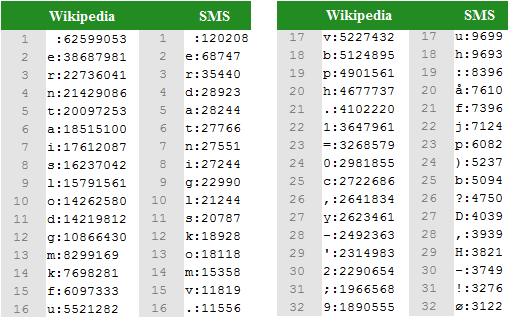
\includegraphics{Billeder/wikiVsSms.png}
\caption {Oversigt over de øverste 32 tegn.}
\label{wikiSMS2}
\end{center}
\end{table}


Det gik op for os at vi måtte analysere rigtige SMS beskeder. Snart var 13.000 SMS beskeder indsamlet og klar til analysering. Som forventet rykker tegn der indgår i humørikoner højere op på listen. Det største spring ser vi ved kolon, som rykker fra plads 53 på wikipedia-listen til plads 19 på SMS-listen. Ydermere ser vi at ”H” går fra plads 56 på wikipedia-listen til plads 26 på SMS-listen. Det kan forklares med at mange beskeder starter med ordet ”Hej”. Se eventuelt bilag \ref{wikiAnalyse} og \ref{SMSanalyse}. Alt dette er vi nødt til at tage hensyn til i vores implementering af Huffman algoritmen.

[SAMMENLIGNING AF ANTAL TEGN I ALT]

Eftersom vi  ”kun” har skaffet 13.000 SMS beskeder, kan vi ikke tolke resultatet entydigt. SMS’erne er indhentet fra 4 forskellige personer, hvilket groft sagt betyder at 6.500 SMS’er, altså halvdelen, er skrevet af disse 4 personer. Tallet kan endda vise sig at være endnu højere, da flere af testpersonerne kender hinanden. Dette kan skabe uligheder i resultatet hvis personerne har en speciel måde at skrive på, altså visse tegn ligger muligvis højere end de ville hvis vi havde fået skaffet beskeder fra flere end 4 personer. Det kan være tegn som ”*”, der bruges i humørikoner. På vores resultatliste ligger ”*” tegnet på plads nummer 47 med 1077 forekomster. 905 af disse forekomster er imidlertid kun fra én persons SMS beskeder, hvilket betyder at personen står for over 84\% af forekomsterne af tegnet - langt mere end de optimale 25\%. Det har ikke været muligt at skaffe flere SMS’er, hvilket nok er grundet at ens beskeder kan være meget personlige.

Konklusionen er at man er nødt til at tage højde for tegn der indgår i humørikoner, og nedprioritere visse tegn som ligger højt på wikipedia-listen.
  

   \section{Program}

	\subsection{Dataindsamling}
	\label{SmaaProg}
Før vi kunne analysere SMS-beskeder, Wikipedia artikler eller andet materiale, var vi nødt til at lave to mindre programmer.

Det ene program skulle sørge for at tekststykket der skulle analyseres, ikke indeholdte andet end den rå tekst. Samtlige SMS-beskeder var fyldt med mange andre informationer end selve SMS-beskeden. Informationer som afsenderens telefonnummer, afsendelses tidspunkt og hvad afsenderens navn i telefonbogen. Al denne information måtte sorteres fra, da den ville have indflydelse på resultatet. Vi fik lavet et program der kunne læse XML filerne, den filtype som SMS’erne var gemt som, der kunne vælge kun at læse bestemte tags. I dette tilfælde var det som sagt kun body tagget vi var interesserede i, altså selve SMS-beskeden. Programmet læser alt der står mellem tagget body=”.....” . Vi havde her taget højde for, at der kunne befinde gåseøjne inde midt i beskederne, disse var på forhånd escapet. Efter de reelle beskeder var indlæst, erstatter programmet de XML escapes der måtte være med ASCII escape sekvenser. Herefter kører den de resterende SMS-beskeder igennem på samme vis.

Det andet program var noget mere simpelt. Det læste beskederne igennem fra ende til anden, og talte hvert tegn det stødte på op, til sidst blev tegnene sorteret efter hyppighed, dvs. de tegn der optrådte flest gange i teksten kom øverst.
   
  	 \subsection{Bit-træer}
   	statisk træ
ved analysering

\begin{figure}[hba]
\centering
\begin{tabular}{|c|c|}
\hline
\cellcolor{ForestGreen}\color{white}{\textbf{Tegn}} &
\cellcolor{ForestGreen}\color{white}{\textbf{Frekvens}} \\ 
\hline 
  & 00 \\
\hline
H & 0100000 \\
\hline
, & 0100001 \\
\hline
1 & 01000100 \\
\hline
0 & 01000101 \\
\hline
D & 0100011 \\
\hline
: & 010010 \\
\hline
/ & 010011000 \\
\hline
6 & 0100110010 \\
\hline
7 & 0100110011 \\
\hline
M & 010011010 \\
\hline
* & 010011011 \\
\hline
; & 01001110 \\
\hline
I & 0100111100 \\
\hline
< & 01001111010 \\
\hline
Y & 01001111011 \\
\hline
V & 010011111 \\
\hline
r & 0101 \\
\hline
e & 011 \\
\hline
o & 10000 \\
\hline
k & 10001 \\
\hline
K & 100100000 \\
\hline
c & 100100001 \\
\hline
3 & 100100010 \\
\hline
x & 10010001100 \\
\hline
+ & 10010001101 \\
\hline
R & 1001000111 \\
\hline
? & 1001001 \\
\hline
h & 100101 \\
\hline
u & 100110 \\
\hline
b & 1001110 \\
\hline
S & 10011110 \\
\hline
O & 100111110 \\
\hline
 & 100111111000 \\
\hline
\ & 100111111001000000 \\
\hline
 & 1001111110010000010 \\
\hline
 & 1001111110010000011 \\
\hline
 & 10011111100100001 \\
\hline
& 1001111110010001 \\
\hline
{ & 100111111001001 \\
\hline
 & 100111111001010 \\
\hline
& & 100111111001011 \\
\hline
= & 10011111100110 \\
\hline
% & 100111111001110 \\
\hline
q & 100111111001111 \\
\hline
z & 100111111010 \\
\hline
C & 100111111011 \\
\hline
F & 1001111111 \\
\hline
s & 10100 \\
\hline
l & 10101 \\
\hline
) & 1011000 \\
\hline
N & 101100100 \\
\hline
9 & 1011001010 \\
\hline
8 & 1011001011 \\
\hline
J & 10110011 \\
\hline
. & 101101 \\
\hline
g & 10111 \\
\hline
v & 110000 \\
\hline
y & 11000100 \\
\hline
L & 11000101000 \\
\hline
U & 110001010010 \\
\hline
' & 110001010011 \\
\hline
( & 1100010101 \\
\hline
4 & 1100010110 \\
\hline
5 & 1100010111 \\
\hline
p & 1100011 \\
\hline
i & 11001 \\
\hline
n & 11010 \\
\hline
 & 11011000 \\
\hline
 & 11011001 \\
\hline
! & 11011010 \\
\hline
B & 11011011000 \\
\hline
G & 11011011001 \\
\hline
P & 1101101101 \\
\hline
2 & 110110111 \\
\hline
j & 1101110 \\
\hline
f & 1101111 \\
\hline
t & 11100 \\
\hline
a & 11101 \\
\hline
d & 11110 \\
\hline
- & 11111000 \\
\hline
T & 1111100100 \\
\hline
E & 1111100101 \\
\hline
 & 1111100110000 \\
\hline
W & 1111100110001 \\
\hline
 & 1111100110010000 \\
\hline
 & 11111001100100010 \\
\hline
 & 11111001100100011000 \\
\hline
 & 11111001100100011001 \\
\hline
 & 11111001100100011010 \\
\hline
@ & 11111001100100011011 \\
\hline
^ & 11111001100100011100 \\
\hline
| & 11111001100100011101 \\
\hline
 & 11111001100100011110 \\
\hline
 & 11111001100100011111 \\
\hline
Q & 111110011001001000 \\
\hline
# & 1111100110010010010 \\
\hline
] & 11111001100100100110 \\
\hline
 & 11111001100100100111 \\
\hline
> & 1111100110010010100 \\
\hline
 & 11111001100100101010 \\
\hline
 & 11111001100100101011 \\
\hline
_ & 1111100110010010110 \\
\hline
 & 11111001100100101110 \\
\hline
} & 11111001100100101111 \\
\hline
 & 1111100110010011000 \\
\hline
 & 11111001100100110010 \\
\hline                                                                                                           
& 11111001100100110011 \\
\hline & 11111001100100110100 \\
\hline
~ & 11111001100100110101 \\
\hline
 & 11111001100100110110 \\
\hline
[ & 11111001100100110111 \\
\hline
 & 11111001100100111000 \\
\hline
	 & 11111001100100111001 \\
\hline
 & 11111001100100111010 \\
\hline
$ & 11111001100100111011 \\
\hline
` & 1111100110010011110 \\
\hline
 & 11111001100100111110 \\
\hline
 & 11111001100100111111 \\
\hline
 & 111110011001010 \\
\hline
^[[?1;2 & 1111100110010110 \\
\hline
cZ & 1111100110010111 \\
\hline
X & 11111001100110 \\
\hline
" & 11111001100111 \\
\hline
w & 11111001101 \\
\hline
A & 1111100111 \\
\hline
 & 1111101 \\
\hline
m & 111111 \\
\hline
\end{tabular} 
\caption{Frekvens for tegn i sætningen ''dette er et eksempel''}
\label{tab:huffmantable_new}
\end{figure}


\chapter{Konklusion}

           I dette afsnit bliver der kigget tilbage på problemformuleringen og ser på hvordan spørgsmålene er blevet besvaret, både hvis det viste sig at være positivt eller negativt.

Den første del af problemformuleringen lyder;\\
\emph{Hvordan kan man spare forbrugeren for dobbelt SMS-takst, ved brug af et komprimeringsprogram?}
 
Til at besvare dette spørgsmål blev der udviklet et program, som kan komprimere en tekstbesked ved brug af Huffman-algoritmen. Huffman komprimeringsalgoritmen blev valgt til udviklingen af løsningen, fordi den passede bedst overens med projektets rammer, samt den platform som programmet var rettet imod. Som det ses i afsnittet \ref{resultater} er det lykkedes at komprimere beskeder med over 30 til 40 procent, hvilket betyder at det, med brug af programmet, er muligt at sende to SMS-beskeder som én. På den måde vil brugeren kunne spare SMS-takst, hver gang der skal sendes en SMS på over 160 tegn.
 
Derudover er der også blevet dokumenteret for at problemstillingen er mulig at løse. Der blev vist, at brugen af SMS er fortsat stor, selvom andre mobile enheder, som har tilgang til internet, heriblandt smartphones, med mulighed for at sende e-mails uden tegn begrænsning, stadigvæk overtager mere og mere af markedet. Der blev også vist, at især SMS-taksten til og fra Danmark og bestemte lande er høj i forhold til SMS-taksten mellem Danmark og andre bestemte lande. Derudover så blev der også vist, at SMS-taksten begyndte at stige i nyere tid.
 
Udfra det kan der blive konkluderet at man kan spare brugeren penge ved at komprimere en SMS besked som overstiger tegnbegrænsningen, og dermed gøre en besked der normalt ville tage dobbelt SMS-takst til enkelt SMS-takst. Derudover, måske lidt mindre væsentligt, så kan man også sænke belastningen på det mobile datatrafik netværk, idet Huffman komprimering gør størrelsen på beskeden mindre. Den samlede besparelse på SMS-forbruget, kommer både an på hvor mange SMS'er der sendes og ligeledes an på hvor mange af dem der fylder mere end 160 tegn.

 
Næste del af problemformuleringen lyder;\\
\emph{Hvordan kan man undgå at programmet bliver en belastning for brugeren?} 

Til at besvarer dette spørgsmål så blev det kigget på de forskellige fordele og ulemper der er ved at bruge forskellige komprimeringsalgoritmer, som for eksempel Huffman og PPM. En PPM komprimeringsalgoritme kræver en del mere af den enhed den kører på, i forhold til Huffman, og blev derfor ikke brugt til at udvikle løsningen, men i stedet, blev det bestemt, at den skulle udvikles med en Huffman komprimeringsalgoritme. Derudover blev det også bestemt, at Huffman skulle laves ud fra den statiske model. I forhold til både den dynamiske og den adaptive model, så krævede den statiske model langt mindre af den enhed, som den kørte på, så der derved ikke kom nogen problemer med, at enheden kørte dårligere på grund af programmet. 

Løsningen skulle også gerne være i stand til at køre under SMS-processen, sådan at brugeren af programmet ikke behøver at gøre noget ekstra, for at få SMS beskeden komprimeret eller dekomprimeret. Komprimeringsprocessen skulle gerne ske automatisk, idet brugeren afsender eller modtager en SMS besked. I løsningen er dette ikke tilfældet. Sådan som løsningen er lige nu, så spørger den efter hvorvidt, der skal komprimeres eller dekomprimeres. Løsningen kan derfor ikke køre under SMS-processen sådan at brugeren ikke ligger mærke til komprimeringen.

           \subsection{Perspektivering}
	Hvis projektet skulle laves forfra, så skulle der forsøges at indsamle data om interessenterne for løsningen. Det ville eksempelvis være interessant at vide hvor mange SMS-beskeder de sender, både indenrigs og udenrigs. Derudover ville det selvfølgelig være vigtigt at vide hvor mange af deres SMS-beskeder, der overstiger 160 tegn. Til at indsamle denne kvantitative data, ville en spørgeskemaundersøgelse være en god mulighed. Ved at have denne data, kunne man regne på den faktiske besparelse på SMS-forbrug for et firma eller privatpersoner, hvis de implementerede dette projekts løsning. Herved kunne der blive vurderet, om programmet ville have en effekt af betydning. 

Derudover kunne det også være relevant, at kigge på om løsningen ville påvirke teleselskaberne, og hvorvidt det ville være positivt eller negativt. Spørgsmålet er om teleselskaberne ville miste penge ved at deres kunder sender færre SMS-beskeder, eller om de selv kunne spare penge, hvis løsningen blev implementeret i deres netværk. Derudover kunne man også undersøge i hvilke andre sammenhænge man ellers med fordel kan bruge datakomprimering. For eksempel når man skal lagre filer og ved generel internettrafik. Ud fra det kunne man finde ud af om løsningen kunne være relevant i andre sammenhænge.

Hvis programmet skulle bruges i al almindelighed ville det kræve at alle mobiltelefoner skulle have programmet installeret. Ellers vil en modtager, som ikke har programmet, læse den komprimerede besked, og denne giver ikke megen mening. Dette er nødvendigt fordi løsningen gør brug af et statisk træ, som er et generelt træ for hvor tit tegn forekommer i en tekst. Det vil sige at alle mobiltelefoner skulle opdateres til at indeholde programmet. Hvis man gjorde brug af et dynamisk eller adaptivt træ, så er det stadig en nødvendighed at modtageren har et eller andet installeret, sådan at enheden kan dekomprimere og læse beskeden. Dette er et krav, uanset hvilken form for komprimeringsalgoritme man gør brug af. En måde hvorpå man kan lettere komme omkring denne forhindring, kunne være et fremtidigt mål for programmet.
 
Derudover er det forventet, at komprimerings programmet vil  blive mest udbredt blandt smartphones, idet de har noget lettere tilgang til ny software eller applikationer. Dermed er det ikke sagt, at dette projekts løsning ville være umulig at installere på en mobiltelefon, det ville bare være lidt mere krævende end at downloade en applikation til en smartphone. Et fremtidigt mål kunne derfor være at finde en måde, sådan at det er let at implementere løsningen på både almindelige mobiltelefoner og smartphones. 

Til det nuværende statiske Huffman træ, som bliver brugt til at komprimere SMS beskeder, blev der indsamlet omkring 14.000 SMS beskeder. En mængde på 14.000 SMS beskeder giver et godt træ, som er forholdsvist præcis og tilpasset til skrivestilen ved SMS beskeder. Træet bliver dog kun bedre hvis mængden af SMS bliver større, idet træet bliver mere præcist, og tilpasser sig mere skrivestilen for den generelle bruger, end en håndfuld af personer. Et mål til at forbedre træet kunne derfor være at indsamle langt flere SMS beskeder, samt finde en måde at indsamle SMS beskeder som tager højde for brugerens privatliv.
  
I fremtiden kunne man muligvis overveje, hvorvidt PPM kan blive implementeret. PPM kan blive bygget ovenpå den allerede eksisterende Huffman komprimeringsalgoritme, og derved gøre løsningen langt bedre. Derudover skal der også laves nogle flere overvejelser, om hvor meget regnekraft og plads man har tilgængelige på en mobiltelefon eller smartphone. Det er muligt, at især smartphones har nået et punkt hvor de sagtens kan håndtere tungere programmer, som derfor åbner op for mulige løsninger ved at bruge PPM, og derudover også bruge dynamiske eller adaptive Huffman træer.

%\begin{thebibliography}{99} %Max
\bibliographystyle{plain}
\bibliography{Referencer}
%\end{thebibliography}

\chapter*{Bilag}
\begin{figure}[H]
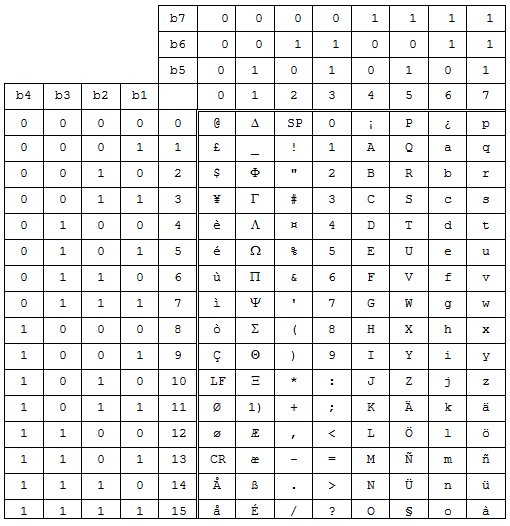
\includegraphics []{Billeder/tegnsaet.png}
\caption {Her ses skemaet for bit 7 tegnsættet. Ved 0x1b ses tegnet 1), der er et escape tegn til den ekstra tabel, som ses på figur \ref{tegnsaet2}}
\label {tegnsaet}
\end{figure}

\begin{figure}[H]
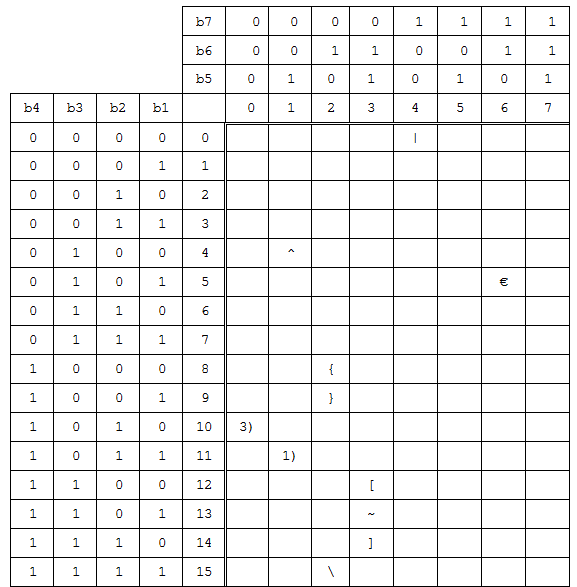
\includegraphics []{Billeder/tegnsaet2.png}
\caption {Den ekstra tabel for bit 7 tegnsaettet. Det samme tegn 1), er her et escape tegn som er reserveret hvis en ny ekstra tabel introduceres. Tegnet 3) er et form feed tegn, som er et escape tegn der starter en ny side.}
\label {tegnsaet2}
\end{figure}

\begin{figure}[H]
\centering
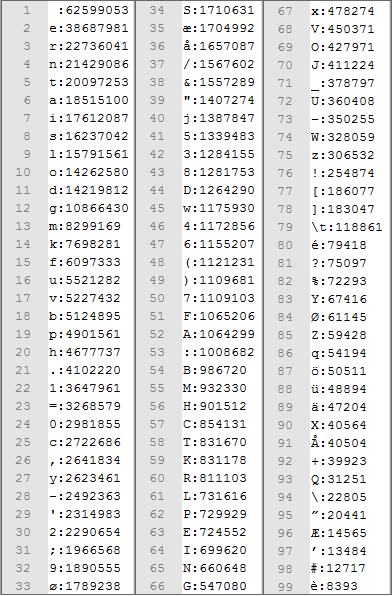
\includegraphics []{Billeder/wikiBilag.png}
\caption {Tabellen viser top 100 over mest brugte tegn i over 340.000 danske Wikipedia artikler.}
\label {wikiAnalyse}
\end{figure}

\begin{figure}[H]
\centering
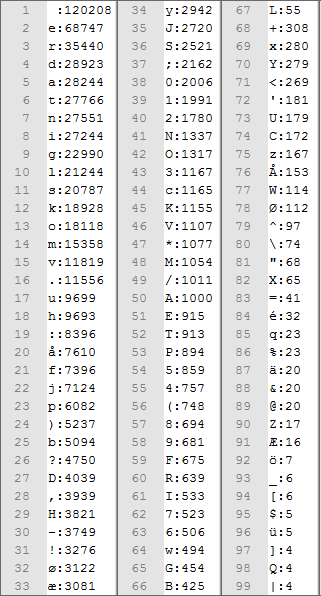
\includegraphics []{Billeder/SMSbilag.png}
\caption {Figuren viser top 100 over mest brugte tegn fra vores SMS analyse af over 13.000 SMS beskeder.}
\label {SMSanalyse}
\end{figure}


\end{document}
